%**********************************************************************
% Base layout + including standard packages
%**********************************************************************
\documentclass[a4paper,12pt]{report}

% allows direct input of special chars
\usepackage[utf8]{inputenc}  

%**********************************************************************
% YOUR SETTINGS - START
%**********************************************************************

% About your study degree programme
\def \study{MSD} % possible options: 
          % ITM ... for BA in Software Design and Cloud Computing (vz vollzeit / ft full-time)
          % SWD ... for BA in Software Design and Cloud Computing (bb berufsbegleitend / pt part-time)
          % MSD ... for BA in Mobile Software Development
          % IRM ... for MA in IT-Recht and Management
          % IMS ... for MA in IT and Mobile Security

% More about you and your thesis:
\def \title{Optimierung von Datenströmen zwischen Frontend und Backend: 
	gRPC im Vergleich zu REST und GraphQL}
\def \subtitle{}
\def \yourName{Michael Mühlberger}
\def \yourIdentifier{<1700000017>} % Used for Seminar Work / Projektarbeit ONLY
\def \yourPlace{Kapfenberg}
\def \submissionDate{Juni 2025}  % month year. e.g. June 2017
\def \yourAdvisor{DI MA Michael Ulm}  


\def \thisDocumentIsA{Thesis} % possible options:
                    % Thesis  .... for Master's Thesis   / Masterarbeit
                    % Thesis  .... for Bachelor's Thesis / Bachelorarbeit
                    % Seminar .... for Seminar Work      / Seminararbeit
                    % Project .... for Project Work      / Projektarbeit

% ITM/SWD/IRM: you could possibly write in German.
\def \yourLanguage{german} % possible options:
                 % english
                 % german

%**********************************************************************
% YOUR SETTINGS - END
%**********************************************************************



% LaTeX preamble = include a lot of packages, configure latex settings
%**********************************************************************
% Various LaTeX packages
%**********************************************************************


% programming (branching) logic
\usepackage{ifthen}

% you might need some mathematical expressions:
\usepackage{amsmath}

% with package babel we allow to use language english and german
\usepackage[english,german]{babel}


% permits to set space between lines
\usepackage{setspace}  	

% ensure proper appearance of all fonts in pdf:
\usepackage[T1]{fontenc}

% lmodern after T1 fontenc (_may_ be required)
% lmodern = Latin Modern fonts
%\usepackage{lmodern}  	

%\usepackage{times} -- obsolete; use:
% Times as default text font, maths support
\usepackage{mathptmx}  	
% provides bold font (required for syntax highlighting in listings)
\usepackage{courier}  	

% enables table cells to span multiple rows
\usepackage{multirow}  
% paragraphs: no indentation at beginning, but spacing between  
\usepackage{parskip}  	

% for figures
\usepackage[pdftex]{graphicx}
% implicit file name extensions for embedded figures 
% so we do not need to specify the extension on inclusion
\DeclareGraphicsExtensions{.pdf,.jpg,.png}

% for flexible tables (e.g. auto resizing to page width) 
%     e.g.: { | l | l | X | }
\usepackage{tabularx}

%**********************************************************************
% Including non-standard packages
%**********************************************************************

% abbreviations are written in full length on first time usage
% e.g. with \acro{UX}{User Experience} 
%    \ac{UX} first time: User Experience (UX)
%    \ac{UX} later:      UX 
\usepackage{acronym}

% http://en.wikibooks.org/wiki/LaTeX/Colors
\usepackage[usenames,dvipsnames,table]{xcolor}
% we define a few custom colors  
\definecolor{gray20}{gray}{0.8}
\definecolor{gray5}{gray}{0.95}
\definecolor{olivegreen30}{RGB}{155,187,89}  

\usepackage{alltt}

% for code snippets, embedded as "listings"
\usepackage{listings}
% we set a few defaults below with \lstset:

  
% the page layout (geometry), 
% as defined by FH guidelines (2.3 Formale Gestaltung):
\usepackage[top=3cm, 
            bottom=3cm, 
            left=3.5cm, 
            right=3cm]
           {geometry}

% superscript st first,
%             nd second
%             rd third
%             th fourth,...
\usepackage[super]{nth}     % 1st, 2nd, 3rd,...

%\usepackage{paralist}   	% inline lists
%\usepackage{mdwlist}
\usepackage{enumitem}

% e.g. for "floating" listings (no fixed anchor in text)
\usepackage{float}     
\floatstyle{plain}
\restylefloat{figure}
% e.g. to show two (floating) images side-by-side
\usepackage{subfig}

% add copyright information to figures
\usepackage{copyrightbox} 



% symbols such as \texttimes and \texteuro
\usepackage{textcomp}  
% math. symbols from the American Mathematical Society  
%\usepackage{amssymb}  	


% chapter heading styles
% see 3.2 The Chapter Lenny at
%         https://ctan.org/pkg/fncychap
\usepackage[Lenny]{fncychap}  

% for \enquote, \textquote, \blockquote...
\usepackage[autostyle]{csquotes}       

% how to create simple helper commands (LaTeX "macros"):
% e.g. red-coloured text when using ...
%      \TODO{Do not forget to add further references}
\newcommand{\TODO}[1]
{
{\textcolor{red}{[TODO: #1]}}
}


% Create/style more complex new commands:
% e.g. \chapquote{Phone home!}{by E.T.}
% BEGIN: chapquote
\newcommand{\chapquote}[2]  
{%
\begin{quote}
\emph{%
``#1''%
}%
\begin{flushright}
{\scriptsize \sffamily [#2]}%
\end{flushright}
\end{quote}
}
% END: chapquote



% Biblatex = bibliography for LaTeX
% ---------------------------------------------------------------------
% context sensitive quotation; recommended for usage with Biblatex
\usepackage{csquotes}  	
% Note: \date, \origdate, \eventdate, and \urldate 
%       require "yyyy-mm-dd" format,
%       so "dd" or "mm-dd" may be omitted
\usepackage[backend=biber,
            urldate=long,  	        % [Feb. 8, 2027]
                                    %                  default: short 
                                    %                  e.g. 08/15/2010
            style=authoryear-icomp, % Harvard citation style    
                                    %   author, year: ... (cf. Batina et al., 2012, p. 317) 
                                    %   icomp: compact & ibidem: ... see (cf. ibid., p. 317) 
                                    %   see: https://tug.ctan.org/info/biblatex-cheatsheet/biblatex-cheatsheet.pdf 
            backref,                % if you like (cit. on p. 2)
            % sorting=nty, 	        % this is default: sort by name,
                                    %                  title, year
            % sortlocale=de_DE,     % set according to your needs
            natbib=true,  	        % use "natbib"-compatible citation
                                    %                  commands
                                    % do _not_ use package natbib!
            maxbibnames=1000,  	    % show all authors in the 
                                    %                  bibliography
            % ibidpage=true,        % this is default for ibid / 
                                    %                  ebd ("ebenda")                        
            giveninits=true,        % E. B. White instead of Elwyn Brooks White
            uniquename=minyearfull, % Reference Authors with same lastname without initials 
                                    % (otherwise set to  "init")
]{biblatex}

% using & instead of "and"
\renewcommand*\finalnamedelim{\addspace\&\space}

% We enforce strict Harvard style: 
% The URL date default is "(Visited on ...);" => so:
%     BibTeX entries such as:
%      url = {http://...},
%      urldate = {2015-05},
%      urldate = {2015},
%      urldate = {2015-05-17},
%     shall be printed as
%      Available from: <http://...> [May 17, 2015]
\DeclareFieldFormat{urldate}{\mkbibbrackets{#1}}
\ifthenelse{\equal{\yourLanguage}{german}}{
  % for language = german: 
  % [online ] https://dl.acm.com/paper3.pdf [17. Mai 2015]
  \DeclareFieldFormat{url}{[online]\space \url{#1}}
}{ % else: 
   % default language = english
   % Available from: https://dl.acm.com/paper3.pdf [May 17, 2015]
  \DeclareFieldFormat{url}{Available\space from\addcolon\space \url{#1}}
}



% ---------------------------------------------------------------------
% !!
% hyperref should be last package loaded
% !! 
\usepackage[  	              
    pdftitle={\title},
    pdfsubject={\thisDocumentIsA},
    pdfauthor={\yourName},
    pdftex,  	              % driver
    breaklinks,  	          % permits line breaks for long links
    bookmarks,  	          % create Adobe bookmarks
    bookmarksnumbered,        % ... and include section numbers
    linktocpage,  	          % the page number (not the text) is link on TOC
    colorlinks,  	          % 
    linkcolor=black,          % normal internal links;
    anchorcolor=black,        % don't make scientific papers too colourful
    citecolor=black,
    urlcolor=blue,  	      % blue is quite common for urls
    pdfstartview={Fit},       % "Fit" fits the page to the window
    pdfpagemode=UseOutlines,  % open bookmarks in Acrobat
    plainpages=false,         % avoids duplicate page number problem
    pdfpagelabels,
  ]{hyperref}

% we break our rules from above and specify another package AFTER hyperref
% allow to specify multiple refs at once, using \Cref{ }
% e.g. \Cref{lst:hello,lst:closure}
\usepackage{cleveref}


%**********************************************************************
% A hack to allow the urls to break on some more characters
%**********************************************************************

% Uncomment, if you want to break URLs at . @ / ! _ | % ; > .... 
%\def\UrlBigBreaks{\do\.\do\@\do\\\do\/\do\!\do\_\do\|\do\%\do\;\do\>\do\]%
% \do\)\do\,\do\?\do\'\do\+\do\=\do\#\do\:\do@url@hyp}

% Uncomment, if you want to break URLs at 123456789 
%\def\UrlBreaks{\do\1\do\2\do\3\do\4\do\5\do\6\do\7\do\8\do\9}

% Uncomment, if you want to break URLS at abcde....xyz and ABCDE....XYZ  
%\def\UrlBreaks{\do\a\do\b\do\c\do\d\do\e\do\f\do\g\do\h\do\i\do\j\do\k\do\l%
%               \do\m\do\n\do\o\do\p\do\q\do\r\do\s\do\t\do\u\do\v\do\w\do\x%
%               \do\y\do\z%
%               \do\A\do\B\do\C\do\D\do\E\do\F\do\G\do\H\do\I\do\J\do\K\do\L%
%               \do\M\do\N\do\O\do\P\do\Q\do\R\do\S\do\T\do\U\do\V\do\W\do\X%
%               \do\Y\do\Z%
%}

% To break URLs in the bibliography
% "bib url lc penalty" will add a breakpoint after all lowercase letters. 
\setcounter{biburllcpenalty}{7000} 
% "bib url uc penalty" will add a breakpoint after all lowercase letters.
\setcounter{biburlucpenalty}{8000} 



%**********************************************************************
% Layout adjustments
%**********************************************************************

% page layout (header/footer and page numbers) 
\pagestyle{headings} % options:
         % headings
         % fancy
         % empty

% Optimise headers / footers
%   when printing the first page of a (numbered) chapter 
%   suppress the page number (on center bottom)
\newcommand{\chapterstart}{\thispagestyle{empty}}
%   when printing the first page of the bibliography
%   suppress the page number (on center bottom)
\AtBeginBibliography{\thispagestyle{empty}}

         
% settings for structure and numbering 
%  we allow three levels within text:  1.2.1 
\setcounter{secnumdepth}{3}
%  but we show two levels in TOC: 1.2
\setcounter{tocdepth}{1}



% command "\chapterend" to close a chapter 
% (flush, i.e. print remaining figures and tables)
\newcommand{\chapterend}
           {\newpage{
              \pagestyle{empty}
               \cleardoublepage
             }
           }

% footnotes: no indent, hanging
\usepackage[hang,flushmargin]{footmisc}

% new environment for smaller paragraphs
% e.g. \begin{spar}A paragraph with some indentation.\end{spar}
\newenvironment{spar}
{\begingroup \leftskip 0.7cm \rightskip\leftskip}
{\par \endgroup}
% ^^^ must be set here (or use empty line)


%**********************************************************************
% LaTeX macros and commands to style the ISBN and color code listings
%**********************************************************************



% Bibliography: distinguish between cited and non-cited entries
%               so it is possible to show non-cited entries as 
%               Further Readings
\DeclareBibliographyCategory{cited}
\AtEveryCitekey{\addtocategory{cited}{\thefield{entrykey}}}

% Bibliography: we create links for given ISBN
\DeclareFieldFormat{isbn}{\isbn{#1}}
\newcommand{\isbn}[1]
{%
{%
\ifpdf
{\small ISBN}
\href{https://isbnsearch.org/isbn/#1}{#1}%
\else
{\small ISBN}
#1%
\fi
}%
}


% You might define support for further programming languages
% when using listings
\usepackage{color}
\definecolor{lightgray}{rgb}{.9,.9,.9}
\definecolor{darkgray}{rgb}{.4,.4,.4}
\definecolor{purple}{rgb}{0.65, 0.12, 0.82}
\lstdefinelanguage{JavaScript}{
  keywords={break, case, catch, continue, debugger, default, delete, do, else, false, finally, for, function, if, in, instanceof, new, null, return, switch, this, throw, true, try, typeof, var, void, while, with},
  morecomment=[l]{//},
  morecomment=[s]{/*}{*/},
  morestring=[b]',
  morestring=[b]",
  ndkeywords={class, export, boolean, throw, implements, import, this},
  keywordstyle=\color{blue}\bfseries,
  ndkeywordstyle=\color{darkgray}\bfseries,
  identifierstyle=\color{black},
  commentstyle=\color{purple}\ttfamily,
  stringstyle=\color{red}\ttfamily,
  sensitive=true
}

\lstset{numbers=left, 
        basicstyle=\footnotesize\ttfamily,  
        showstringspaces=false,
        % numbers=none           % disable line numbering
        captionpos=b,            % caption at bottom
        breaklines=false, 
        numbersep=5pt,           % space for numbers
        caption={Listing subtitles could and should contain whole sentences
                 describing the important aspect of the listing.}, 
        float=tbhp,             % float listing to top/bottom/here/page
        language=JavaScript,     % Python Ruby SQL ksh erlang ...
        frame=single,
        breaklines=true,         % break long source code lines, add arrow
        postbreak=\mbox{\textcolor{red}{$\hookrightarrow$}\space},
        basewidth={0.55em}, 
}



%**********************************************************************
% Special hyphenation rules
%**********************************************************************

\hyphenation{JOANNEUM}  	% extend to your needs

%**********************************************************************
% Different settings for ITM / SWD / IRM / IMS
%**********************************************************************


% ITM = Internettechnik
% SWD-CC(vz) was formerly called : "Internettechnik"
% ------------------------
\ifthenelse{\equal{\study}{ITM}}{
  \def \theStudyProgramme {Software Design and Cloud Computing}
  \def \isBachelorThesis {}
}
%\fi

% SWD = Software Design
% SWD-CC(pt) was formerly called : "Software Design"
% ------------------------
\ifthenelse{\equal{\study}{SWD}}{
  \def \theStudyProgramme {Software Design and Cloud Computing}
  \def \isBachelorThesis {}
}

% MSD = Mobile Software Development
% ------------------------
\ifthenelse{\equal{\study}{MSD}}{
  \def \theStudyProgramme {Mobile Software Development}
  \def \isBachelorThesis {}
}


% IRM = IT-Recht & Management
% -------------------------------
\ifthenelse{\equal{\study}{IRM}}{
  \def \theStudyProgramme {IT-Recht \& Management}
  \def \isMasterThesis {}
}

% IMS = IT & Mobile Security
% ------------------------------
\ifthenelse{\equal{\study}{IMS}}{
  \def \theStudyProgramme {IT \& Mobile Security}
  \def \isMasterThesis {}
}


 

% Add one (or multiple) file(s) with bibliography entries:
%   here "thesis.bib" i.e. pdflatex sets \ to 'thesis'
%   the name specified when running pdflatex
%   \addbibresource{thesis.bib}
\addbibresource{thesis.bib}





\begin{document}
%**********************************************************************
% Structure of thesis: inclusion of chapters
%**********************************************************************
\ifthenelse{\equal{\yourLanguage}{german}}{
  \selectlanguage{german}
}{ % else: default language = english
  \selectlanguage{english}
}




\ifthenelse{\equal{\thisDocumentIsA}{Thesis}}{  
  % a title page is included for BA/MA Thesis only
  %**********************************************************************
% right side, if two-sided
\chapterend

\begin{titlepage}

\begin{center}
% scale image according to the actual logo you use
% official JPG ist way too large, so [height=2.5cm] is required
% official EPS, converted to PDF:

\includegraphics[height=1cm]
                {images/logo_FHJ_100mm_cmyk.pdf}
\hfill

% the actual title
\mbox{}\vfill

  \large

  {\huge\bf \title \par}
  \subtitle
  \vspace{2.0cm}
  
\ifdefined\isMasterThesis % MA

  \ifthenelse{\equal{\yourLanguage}{german}}{ % German Version 

   {\bf Masterarbeit}\\
    zur Erlangung des akademischen Grades\\
   
    \ifthenelse{\equal{\study}{IRM}}{ % IRM Master of Arts
  
      {\bf Master of Arts in Business (MA)}\\
      eingereicht am\\
      Fachhochschul-Studiengang {\bf \theStudyProgramme \\}
  
    }{  % else: IMS = Master of Science
      
      {\bf Master of Science in Engineering (MSc)}\\
      eingereicht am\\
      Fachhochschul-Studiengang {\bf \theStudyProgramme \\}
      
   }

  }{ % English Version 

    {\bf Master's Thesis}\\
    submitted in conformity with the requirements for the degree of\\
   
    \ifthenelse{\equal{\study}{IRM}}{ % IRM Master of Arts
  
      {\bf Master of Arts in Business (MA)}\\
      Master's degree programme {\bf \theStudyProgramme \\}
  
    }{  % else: IMS = Master of Science
      
      {\bf Master of Science in Engineering (MSc)}\\
      Master's degree programme {\bf \theStudyProgramme \\}
      
   }

  } 
\else % BA
  
  \ifthenelse{\equal{\yourLanguage}{german}}{ % German Version 
  
  {\bf Bachelorarbeit}\\
  zur Erlangung des akademischen Grades\\
  {\bf Bachelor of Science in Engineering (BSc)}\\
  
  eingereicht am\\
  Fachhochschul-Studiengang {\bf \theStudyProgramme \\}

  }{ % English Version 
  
  {\bf Bachelor's Thesis}\\
  submitted in conformity with the requirements for the degree of\\
  {\bf Bachelor of Science in Engineering (BSc)}\\
  Bachelor's degree programme {\bf \theStudyProgramme \\}

  }

\fi
  
  \vspace{0.5cm}

 FH JOANNEUM  (University of Applied Sciences), Kapfenberg

  \vspace{1.5cm}

  \mbox{}

  \ifthenelse{\equal{\yourLanguage}{german}}{ % German Version

  {\bf Betreuer/in: \yourAdvisor\\
   % Zweit-/Firmenbetreuer/in: <Vorname Zuname; Firmenname>

  Eingereicht von: \yourName
  }
  
  
  }{ % English Version 

  {\bf Supervisor: \yourAdvisor\\ 
  % second supervisor: <firstname lastname; company>

  Submitted by: \yourName
  }
  
  }

  \vspace{1.5cm}

   \submissionDate
  
  \vspace{1.5cm}
% \TODO{Specify the title, sub title, place, date, study, language, 
	% your name, and advisor in the main \emph{thesis.tex} file.\\
	% Finally, remove all \emph{TODOs} within your \LaTeX source code.}


\end{center}

\vfill\mbox{}


\end{titlepage}



%**********************************************************************

}{ 
  \ifthenelse{\equal{\thisDocumentIsA}{Seminar}}{ 
    % Seminar Work (se)
    %**********************************************************************
% right side, if two-sided
\chapterend

\begin{titlepage}

\begin{center}
% scale image according to the actual logo you use
% official JPG ist way too large, so [height=2.5cm] is required
% official EPS, converted to PDF:

\includegraphics[height=1cm]
                {images/logo_FHJ_100mm_cmyk.pdf}
\hfill

% the actual title
\mbox{}\vfill

  \large

  {\huge\bf \title \par}
  \subtitle
  \vspace{2.0cm}
  
  \ifthenelse{\equal{\yourLanguage}{german}}{ % German Version 

   {\bf Seminararbeit}
   

  }{ % English Version 

    {\bf Seminar Work}
  } 

  
  \vspace{0.5cm}

 FH JOANNEUM  (University of Applied Sciences), Kapfenberg

  \vspace{1.5cm}

  \mbox{}

  \ifthenelse{\equal{\yourLanguage}{german}}{ % German Version

  {\bf Betreuer/in: \yourAdvisor\\
   % Zweit-/Firmenbetreuer/in: <Vorname Zuname; Firmenname>

  Eingereicht von: \yourName\\
  Personenkennzahl: \yourIdentifier}
  
  
  }{ % English Version 

  {\bf Supervisor: \yourAdvisor\\ 
  % second supervisor: <firstname lastname; company>

  Submitted by: \yourName\\
  Personal identifier: \yourIdentifier}
  
  }

  \vspace{1.5cm}

   \submissionDate
  
  \vspace{1.5cm}
  \TODO{Specify the title, sub title, place, date, study, language, your name, advisor and your id in the preamble in file thesis.tex.}

\end{center}

\vfill\mbox{}


\end{titlepage}



%**********************************************************************

  }{
    % Project Work (pw)
    %**********************************************************************
% right side, if two-sided
\chapterend

\begin{titlepage}

\begin{center}
% scale image according to the actual logo you use
% official JPG ist way too large, so [height=2.5cm] is required
% official EPS, converted to PDF:

\includegraphics[height=1cm]
                {images/logo_FHJ_100mm_cmyk.pdf}
\hfill

% the actual title
\mbox{}\vfill

  \large

  {\huge\bf \title \par}
  \subtitle
  \vspace{2.0cm}
  
  \ifthenelse{\equal{\yourLanguage}{german}}{ % German Version 

   {\bf Projektarbeit}
   

  }{ % English Version 

    {\bf Project Work}
  } 

  
  \vspace{0.5cm}

 FH JOANNEUM  (University of Applied Sciences), Kapfenberg

  \vspace{1.5cm}

  \mbox{}

  \ifthenelse{\equal{\yourLanguage}{german}}{ % German Version

  {\bf Betreuer/in: \yourAdvisor\\
   % Zweit-/Firmenbetreuer/in: <Vorname Zuname; Firmenname>

  Eingereicht von: \yourName\\
  Personenkennzahl: \yourIdentifier}
  
  
  }{ % English Version 

  {\bf Supervisor: \yourAdvisor\\ 
  % second supervisor: <firstname lastname; company>

  Submitted by: \yourName\\
  Personal identifier: \yourIdentifier}
  
  }

  \vspace{1.5cm}

   \submissionDate
  
  \vspace{1.5cm}
  \TODO{Specify the title, sub title, place, date, study, language, your name, advisor and your id in the preamble in file thesis.tex.}

\end{center}

\vfill\mbox{}


\end{titlepage}



%**********************************************************************

  }
}


% Anmerkung: 
%    NUR gesperrte Arbeiten werden gedruckt und benötigen eine 
%    Eidesstattliche Erklärung / Signed Declaration
%\include{chapters/02_declaration} 


%**********************************************************************

%---------------------------------------------------
% NOTE:
% An English version of the abstract is always required 
% (even for German BA/MAs).
%---------------------------------------------------

% right side/flush
\chapterend

\begin{titlepage}

\begin{otherlanguage}{english} 

\begin{abstract} % Abstract
\label{abstract_english}
While gRPC is a well-known and used API approach for service-to-service communication in microservice architecture with high performance requirements, gRPC-Web is still less common on the web. The performance benefits of gRPC, are primarily due to binary Protocol Buffers (Protobuf) serialization format and HTTP/2 multiplexing.
Since most browsers do not support the full set of HTTP/2 features, gRPC-Web cannot fully leverage these advantages. Therefore, REST and GraphQL still remain the dominant web API approaches for web clients.
The goal of the Bachelos thesis is to evaluate how gRPC-Web performs compared to REST and GraphQL with respect to latency, efficiency and resource usage and to identify scenarios in which using gRPC-Web for frontend-backend communication is suitable.
The methodology combines a theoredical analysis with an experimental evaluation using a custom-built prototype. The prototype implements several services that cover typical web payloads (e.g.text or media data) and supports tests both in a browser-based web client and a microservice scenario. The measurement series includes single and parallel requests, cross-browser comparison and a contrast between browser-based frontend-backend communication an service-service communication in the microservice scenario.
Measurements show that, in the browser context, gRPC-Web is not a viable performance-oriented replacement for REST or GraphQL. Especially for large media payloads, REST outperforms both gRPC-Web and GraphQL. Although the theoretical analysis showed that Protocol Buffers more efficient than JSON, these advantages were not measurable. This is due to the limited availability of HTTP/2 features in browsers and the additional proxy/translation layer which is required by gRPC-Web. Another disadvantage compared to REST and GraphQL is, that gRPC-Web is harder to learn and has has less documentation, tools and community support.
Overall gRPC still remains the best option for service-to-service communication in microservice architectures, particularly under high request rates and high performance requirements, the use of gRPC-Web in browsers is just useful, when an existing gRPC backend needs to be exposed to browsers. Improved browser support for HTTP/2 and HTTP/3 could change this assessment in the future.


\end{abstract}

\end{otherlanguage}


\end{titlepage}


%---------------------------------------------------
% NOTE:
% A German version of the abstract "Zusammenfassung"
% is always required.
%---------------------------------------------------

\begin{titlepage}

\begin{otherlanguage}{german}

\begin{abstract}  % Zusammenfassung
\label{abstract_german}

Während gRPC bereits als etablierter Standard für die Service-zu-Service in Microservice-Architekturen gilt, ist gRPC-Web im Web-Kontext weniger verbreitet. Die Leistungsvorteile von gRPC basieren insbesondere auf der binären Protobuf-Serialisierung und HTTP/2-Multiplexing. Da Browser wichtige HTTP/2-Features nur eingeschränkt unterstützen, kann gRPC-Web diese Vorteile nicht vollständig nutzen. Im Browserumfeld dominieren daher weiterhin REST und GraphQL als etablierte Web-API-Ansätze.
Diese Bachelorarbeit befasst sich mit den Fragen, wie sich gRPC-Web im Vergleich zu den etablierten Web-Technologien REST und GraphQL auf Latenz, Effizienz und Ressourcennutzung in der Frontend-Backend-Kommunikation zwischen einem Web-Client und einem Web-Server auswirkt und unter welchen Bedingungen der Einsatz von gRPC für die Frontend-Backend-Kommunikation sinnvoll ist.
Für die Beantwortung dieser Fragen wird ein kombinierter methodischer Ansatz gewählt: eine theoretischen Analyse und eine experimentelle Evaluation anhand eines eigens entwickelten Prototyps, der die End-zu-End Latenz aus Sicht des Frontend Clients misst. 
Der Prototyp implementiert mehrere Services, die typische Web-Payloads (wie Text- und Mediendaten) abdecken, und Tests sowohl im Browser (Web-Client) als auch in einem Microservice-Szenario (Konsolen-Client). Basierend darauf werden Messreihen mit Einzel- und Parallelenabfragen durchgeführt, verschiedene Browserumbebungen verglichen und die Frontend–Backend-Kommunikation im Browser der Service-zu-Service-Kommunikation im Microservice-Szenario gegenübergestellt.
Die Messungen deuten darauf hin, dass gRPC-Web im Browserumfeld nicht mit den etablierten Web-API-Ansätzen REST und GraphQL konkurrenzfähig ist. Die in der Theorie erwarteten Performanceverbesserungen durch Protobuf konnten durch die Prototypen im Browser nicht bestätigt werden. Grund dafür sind die fehlenden HTTP/2-Features im Browser und der zusätzliche Übersetzungsschritt von gRPC zu gRPC-Web. Zusätzlich ist der Erlernbarkeit von gRPC-Web  im Vergleich zu etablierten Technologien wie REST komplexer und es stehen weniger Dokumentation, Tools und Community-Ressourcen zur Verfügung. Vor allem bei großen Binärdaten erwies sich REST im Browser als robuster.
Insgesamt empfiehlt sich gRPC weiterhin vor allem für Service-zu-Service Szenarien mit hoher Requestfrequenz während eine Implementierung von gRPC-Web nur dann sinnvoll ist, wenn bereits ein gRPC-basiertes Backend besteht. Bei verbesserter Browser-Unterstützung für HTTP/2 oder HTTP/3 könnte sich dies künftig ändern. 


\end{abstract}

\end{otherlanguage}

\end{titlepage}

%**********************************************************************


% optional:
%%**********************************************************************

% Optional: add acknowledgement
\chapterend

\begin{titlepage}

\begin{center}\large\bf

\ifthenelse{\equal{\yourLanguage}{german}}{ % German Version
 Danksagung 
}{ % English Version
 Acknowledgement 
}
\end{center}
Your text here\ldots
\TODO{Optionally, you might say thank you or give credits to someone.}

\end{titlepage}


%**********************************************************************
 

\chapterend

\pagenumbering{roman}  	% roman page numbers for title pages


\tableofcontents            % TOC = Table-of-Contents

% OPTIONALLY, adding single entries (LoF, LoT, LoL) to TOC: 

% Adding entry LoF "List of Figures / Abbildungsverzeichnis" to TOC
\clearpage
\addcontentsline{toc}{chapter}{\listfigurename} 
\listoffigures

% Adding entry LoT "List of Tables / Tabellenverzeichnis" to TOC
\clearpage
\addcontentsline{toc}{chapter}{\listtablename}
\listoftables 

% Adding entry LoL "List of Code Snippets" to TOC
% \clearpage
% \addcontentsline{toc}{chapter}{List of Code Snippets}
% \lstlistoflistings

\chapterend





\pagenumbering{arabic}  % ... for ordinary chapters
\onehalfspacing



% remove this, when starting to write your thesis:
%%%%%%%%%%%%%%%%%%%%%%%%%%%%%%%%%%%%%%%%%%%%%%%%%%%%%%%%%%%%%%%%%%%%%%%%%%%%%
\chapter{ Einleitung }
\label{chap:info_REMOVE_ME}
%%%%%%%%%%%%%%%%%%%%%%%%%%%%%%%%%%%%%%%%%%%%%%%%%%%%%%%%%%%%%%%%%%%%%%%%%%%%%
\chapterstart

\section{Motivation}
Bei Echtzeitanwendungen wie Chat-Applikationen oder Streaming Diensten werden oft große Datenmengen ausgetauscht. Dabei ist eine effiziente Übertragung der Daten essenziell, damit die Latenz so klein wie möglich bleibt. Eine Methode um dies in einem Softwareprojekt zu implementieren ist das gRPC Remote Procedure Call (gRPC) Framework, indem die Daten binär kodiert mittels dem Hypertext Transfer Protocol (HTTP)/2 Protokoll übertragen werden. (\parencite{gRPCAbout})
Während sich diese Strategie für Datenströme in Backend-Architekturen und insbesondere in Microservice-Umgebungen bereits etabliert hat, ist eine nahtlose Implementierung von gRPC in Frontendanwendungen in Web-Browsern noch nicht möglich. Hauptgrund dafür, sind fehlende HTTP/2-Features in den Browsern (z. B. bidirektionales Streaming) welche eine Voraussetzung für eine Implementierung von gRPC darstellen. Eine Abhilfe dafür ist gRPC-Web, eine angepasste Variante von gRPC, die dafür entwickelt wurde, gRPC auch in Webbrowsern nutzbar zu machen. Während durch die Verwendung von gRPC-Web einige Features verloren gehen, bleiben auch wichtige Vorteile, wie etwa die Nutzung von Protocol Buffers, erhalten. (\parencite{Brandhorst2019}) In der Praxis wird eine gRPC-Übertragung in der Regel nur verwendet, wenn eine effiziente und schnelle Kommunikation besonders wichtig ist. Ziel der Bachelorarbeit ist es zu untersuchen, inwiefern sich gRPC beziehungsweise gRPC-Web auch in Frontend-Anwendungen sinnvoll einsetzen lassen. Hierfür werden verschieden Application Programming Interface (API)-Übertragungsarchitekturen (Representational State Transfer (REST) und Graph Query Language (GraphQL)), welche sich bereits in der Frontend-zu-Backendkommunikation etabliert haben, mit gRPC und gRPC-Web überprüft und verglichen. (\parencite{Ahmad2025}) Der Schwerpunkt liegt auf den Kriterien Latenz, Effizienz und den generellen Vor- und Nachteilen, die beim Einsatz der jeweiligen Technologien zum Vorschein kommen. Die Bewertung erfolgt sowohl auf theoretischer Grundlage als auch anhand einer praktischen Untersuchung.

\section{Forschungsfragen}
Aus der dargestellten Situation und den Einbußen welche mit der Implementierung von
gRPC in Webanwendungen einhergehen, ergibt sich die Motivation, gRPC /
gRPC-Web mit den etablierten API-Ansätzen für die Frontend- zu Backendkommunikation zu vergleichen. Dafür werden im Rahmen der Bachelorarbeit folgende Forschungsfragen untersucht:

\begin{itemize}
	\item Wie wirkt sich die Verwendung von gRPC bzw. gRPC-Web im Vergleich zu REST
	und GraphQL auf die Latenz, Effizienz und Ressourcennutzung in der Frontend-Backend-Kommunikation aus?
	
	\item Unter welchen Bedingungen ist der Einsatz von gRPC für die
	Frontend-Backend-Kommunikation sinnvoller als REST oder GraphQL?
	
\end{itemize}

Diese Forschungsfragen bilden die Grundlage für die theoretische Analyse sowie die
praktische Untersuchung der genannten API-Technologien. Ziel ist es, anhand dieser
Fragen sowohl die Stärken als auch die Schwächen von gRPC-Web in Webumgebungen
zu identifizieren.


\section{Hypothese}
Für eine strukturiertere Herangehensweise werden folgende Hypothesen formuliert, die
die erwarteten Ergebnisse darstellen:

\begin{itemize}
	\item Es wird angenommen, dass die Nutzung von gRPC im Vergleich zu REST und
	GraphQL die Latenz reduziert und die Effizienz erhöht. Vor allem durch das Verwenden
	von Protocol Buffers, ein binäres Serialisierungsformat welches auch
	bei gRPC-Web verwendet wird, ist eine Effizienzsteigerung im Gegensatz zum klassischen JSON-Format zu erwarten, wodurch sich auch beim Datenaustausch bei praktischen Messungen eine geringere Latenz zeigen sollte.
	
	\item Für gRPC-Web wird angenommen, dass sich zwar performancetechnische Vorteile
	ergeben werden, sich die Implementierung in Projekten der Frontendanwendung
	jedoch als komplexer gestalten wird. Demnach wird der Einsatz von gRPC-Web ähnlich vor allem bei Anforderungen mit hohen Datenmengen sinnvoll sein.

	
\end{itemize}

\section{Methodik}
Folgende methodische Herangehensweise wird für die Beantwortung der Forschungsfragen angewendet:

\subsubsection*{Theoretische Analyse:}
\begin{itemize}
	\item Systematische Literaturrecherche der theoretischen Grundlagen.
	\item Ermittlung des aktuellen Stands der Technik auf Basis wissenschaftlicher Publikationen und relevanter Industriestandards.
	\item Vergleich sowie Gegenüberstellung der Vor- und Nachteile der betrachteten API-Architekturen.
\end{itemize}

\subsubsection*{Erstellen eines Prototyps:}
\begin{itemize}
	\item Experimentelle Methodik: Im praktischen Abschnitt der Arbeit wird ein Prototyp
	entwickelt, der die ausgewählten API-Technologien implementiert.
	\item Auf Basis dieses Prototyps werden Messreihen durchgeführt, welche zur Beantwortung der Forschungsfragen beitragen.
\end{itemize}

Basierend auf den theoretisch und praktisch ermittelten Daten, werden anschließend
die Forschungsfragen beantwortet.
\chapterend
     % LaTeX examples  



% Add chapters as required. For example 

%%%%%%%%%%%%%%%%%%%%%%%%%%%%%%%%%%%%%%%%%%%%%%%%%%%%%%%%%%%%%%%%%%%%%%%%%%%%%%
\chapter{Introduction}
\label{chap:intro}
%%%%%%%%%%%%%%%%%%%%%%%%%%%%%%%%%%%%%%%%%%%%%%%%%%%%%%%%%%%%%%%%%%%%%%%%%%%%%
\chapterstart

% Overall problem
%  and why is it relevant 
%  relevant to which target group
% key questions to answer
% your approach, the method (survey, prototype, user tests, ...)
% one/two hypotheses (idea of solution)

Your text here\ldots 
\TODO{Describe the kind of problem at hand? The problem is relevant in which 
context? What does not work well at the moment? 
What do people need? Describe the background, the prerequisites for your 
work. Optionally, add terms and definitions whenever they might not be clear 
to a fellow student. test ~\parencite{Brooks:1975} }

%%%%%%%%%%%%%%%%%%%%%%%%%%%%%%%%%%%%%%%%%%%%%%%%%%%%%%%%%%%%%%%%%%%%%%%%%%%%%
\section{Problem Statement}\label{sec:problem}
%%%%%%%%%%%%%%%%%%%%%%%%%%%%%%%%%%%%%%%%%%%%%%%%%%%%%%%%%%%%%%%%%%%%%%%%%%%%%

Your text here\ldots 
\TODO{What is the overall problem? Give examples. Motivate! Compared to 
existing solutions for the problem at hand, why does someone need a better, 
faster, and somewhat different one?
test }


%%%%%%%%%%%%%%%%%%%%%%%%%%%%%%%%%%%%%%%%%%%%%%%%%%%%%%%%%%%%%%%%%%%%%%%%%%%%%
\section{Research Questions}\label{sec:rq}
%%%%%%%%%%%%%%%%%%%%%%%%%%%%%%%%%%%%%%%%%%%%%%%%%%%%%%%%%%%%%%%%%%%%%%%%%%%%%

Your text here\ldots 
\TODO{Focus on one or two main research questions and detail on them.}

%%%%%%%%%%%%%%%%%%%%%%%%%%%%%%%%%%%%%%%%%%%%%%%%%%%%%%%%%%%%%%%%%%%%%%%%%%%%%
\section{Hypothesis}\label{sec:hypothesis}
%%%%%%%%%%%%%%%%%%%%%%%%%%%%%%%%%%%%%%%%%%%%%%%%%%%%%%%%%%%%%%%%%%%%%%%%%%%%%


Your text here\ldots 
\TODO{State a hypothesis -- a rough idea -- of how you think a solution might 
look like. Explain, how to possibly solve a given problem.}


%%%%%%%%%%%%%%%%%%%%%%%%%%%%%%%%%%%%%%%%%%%%%%%%%%%%%%%%%%%%%%%%%%%%%%%%%%%%%
\section{Method}\label{sec:method} % Materials and Methods
%%%%%%%%%%%%%%%%%%%%%%%%%%%%%%%%%%%%%%%%%%%%%%%%%%%%%%%%%%%%%%%%%%%%%%%%%%%%%

Your text here\ldots 
\TODO{Your structured, academic approach\footnote{Find an extensive 
explanation of how to write a \emph{Method} section 
at \url{http://www.mrcophth.com/publishorperish/methods.html}.} to find a 
solution. When you needed (large) data sets for you work, explain how you 
collected and filtered raw data. 
For the validation (see Section \nameref{chap:evaluation}~\ref{chap:evaluation}) 
you want to describe the criteria for objective measurement already here.
}


% selected methods (experiment, survey, case study, ...):
% 
%  typical analytic settings: "deductive"
%   	(literature survey)
% 		analysis (according to your previously specified criteria) 
%  typical experimental settings: "inductive"
%  		compare system/situation x and y
%  		new combination of a and b leads to c
%		
%  => 
%  design your experiment
%   decide how to observe (measure) and collect (and process) data
%   prototype implementation = "proof-of-concept
%   study process or software product
% ...
%  often, you might include:
%    user testing, heuristic evaluations





\chapterend

   % framing the problem 
                                     % research questions
                                     % hypothesis
                                     % method

%%%%%%%%%%%%%%%%%%%%%%%%%%%%%%%%%%%%%%%%%%%%%%%%%%%%%%%%%%%%%%%%%%%%%%%%%%%%%
\chapter{Theoretische Grundlagen}
\label{chap:intro}
%%%%%%%%%%%%%%%%%%%%%%%%%%%%%%%%%%%%%%%%%%%%%%%%%%%%%%%%%%%%%%%%%%%%%%%%%%%%%
\chapterstart

\section{Frontend und Backend}

Die Arbeit Untersucht die Kommunikation zwischen Frontend zu Backend Komponenten, im industriellen als auch wissenschafltichem Kontext sind diese Begriffe wie folgt definiert:

\chapquote{Das Frontend ist das, was Ihre Benutzer sehen, und enthält visuelle Elemente wie Schaltflächen, Kontrollkästchen, Grafiken und Textnachrichten. Es ermöglicht den Benutzern, mit Ihrer Anwendung zu interagieren. Das Backend sind die Daten und die Infrastruktur, die dafür sorgen, dass Ihre Anwendung funktioniert. Es speichert und verarbeitet Anwendungsdaten für Ihre Benutzer.}
{\cite{awsfrontendbackend}}

Wie aus dieser Definition ersichtlich beinhaltet das Front-End den benutzerspezifischen Teil und das backend den Datenverarbeitungsteil. Im Zuge der Bachelorarbeit werden anschlieden für die Front End Komponente ebenso das Wort „Client“ und für die Backend Komponente das wort „Server“ verwendet.

\section{Serialisierungsformate}
Bei der Übertragung zwischen der Front-End und Back-End Komponente werden Daten ausgetauscht. Da es eine Vielzahl an Technologien gibt, mit denen die jeweiligen Komponenten realisiert werden können, wurden Standards definiert, damit diese sinnvoll und effizient verarbeitet werden können.

\subsection{JSON}
JSON steht für JavaScript Object Notation und ist ein weit verbreitetes, textbasiertes Datenformat, das vorallem wegen einfacher Lesbarkeit und breiter Unterstützung in vielen Programmiersprachen Verwendung findet. Das Format basiert auf einer Schlüssel-Wert Paar Struktur mit einfacher Syntax ( Klammern, Spalten, Doppelpunkte, Kommas ) und kann folgende Datentypen annehmen:

\begin{itemize}
	\item String (Zeichenkette)
	\item Number (Zahl)
	\item Boolean (true/false)
	\item Array (Liste)
	\item Object (Objekt mit weiteren Schl\"ussel-Wert-Paaren)
	\item null (leerer Wert)
\end{itemize}


JSON ist der Standard für REST und GraphQL Schnittstellen.


\subsection{Protocol Buffers}
Protocol Buffer sind ein von Google entwickeltes Serialisierungsformat. Es handelt sich hierbei um ein binäres Serialisierungsformat, das entwickelt wurde um möglichst effizient, mit hoher Performance und mit so wenig Overhead wie möglich (ohne Whitespaces oder Satzzeichen wie bei JSON) Daten zu übertragen und zu verarbeiten. Protocul Buffer sind Plattform unabhängig und mit den meisten gängigen Programmiersprachen kompatibel.

Ein zentraler Bestandteil Protocol Buffer sind dabei plattformunabhängigen .proto Files, die für die Erzeugung definiert werden müssen.

Mit den definierten .proto Files können anschließend mit einem Plattform Abhängigen Protobuf-Compiler-Tool ( z.B. protoc ) Datenobjekte der jeweiligen Programmiersprache generiert werden.


\newpage
\textbf{\underline{Aufbau der .proto Files}}
\newline
Hauptbestandteil der .proto Files sind messages und services.

\begin{verbatim}
	message Person {
		string name = 1;
		int32 id = 2;
		string email = 3;
	}
\end{verbatim}

Messages geben dabei die Struktur der zu übertragenden Nachricht und den jeweiligen Datentypen an und einer Nummer, die beschreibt an welcher Stelle sich das jeweilige Attribut befindet, an. Die Nummerierung der Felder ist wichtig für die Serialisierung.
In Protocol Buffers können unter anderem die gängigsten Datentypen wie int32, int64, float, double, bool sowie string und bytes verwendet werden.

\begin{verbatim}
	service PersonService {
		rpc GetPerson (PersonRequest) returns (Person);
	}
\end{verbatim}

Services geben an, welche Dienste vom Server bereit gestellt werden und welche Datentypen als Parameter bei Aufruf übermittelt und als Rückgabe zurückgegeben werden. Services müssen auf der Seite des zur Verfügung stellenden Dienstes ausimplementiert werden.

Das Protobuf Serialisierungsformat wurde vorallem für die inter-server Kommunikation ( innherhalb der Backend seitigen Kommunikation) entwickelt, im Zuge der Bachelorarbeit wird diese auf die Verwendung in der Frontend zu Backend Kommunikation untersucht.

\subsection{Übertragung binärer Daten (Blob)}:
Für das Übertragen von großen binären Objekten ( wie Bilder, Video, Audiodateien, Dokumente, .. ) wird eine große Menge an binären Daten ( Datentyp: byte) gesendet. Solche großen binären Dateien, die bei der Kommunikation zwischen Client und Server gesendet werden, werden in der Webentwicklung, und vorallem im Frontend wo diese Mediendaten verarbeitet werden sollen, oft als Blob ( Binary Large Object ) bezeichnet. 


\section{Transportprotokolle}
Die eigentlichen Daten, die in Form von Serialisierungsformaten zwischen Frontend und backend ausgetauscht werden, werden mithilfe von Transportprotokollen von dem Client and den Server, und umgekehrt, übermittelt. Das Hypertext Transfer Protocol (http) ist dabei für moderne Webanwendungen das zentrale und verbreitetste Transportprotokoll. Im Kontext der Bachelorarbeit, wird insbesondere auf zwei Versionen von http eingegangen:

\subsection{HTTP/1.1}

http/1 Ist der momentan am weitesten verbreitetste Protokoll für die Kommunikation zwischen Frontend und Backend anwendungen. Es wird von allen Webbrowsern ohne einschränkungen unterstützt und bildet die Grundlage für die API Technologien REST und GraphQL. Das Protokoll funktioniert mittels eines request-responds Prinzips und überträgt die Daten über eine textbasierte Verbindung mittels eines TCP Transportprotokolls. 

\begin{figure}[htbp]
	\centering
	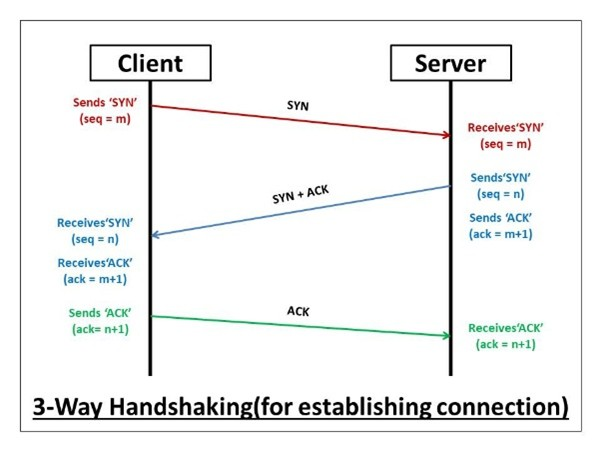
\includegraphics[width=0.7\textwidth]{images/http1_theory.jpg}
	\caption{3-Way Handshake (for establishing TCP connection)}
	\label{fig:threewayhandshake}
\end{figure}

Der Verbindungsaufbau erfolgt dabei mittels eines Transmission Control Protocol  (TCP) – Handshakes, welcher für eine zuverlässige Verbindung zwischen zwei Systemen verwenden wird. Dabei werden in drei Schritten Steuerpakete ausgetauscht:

1. Zuerst sendet der Client ein SYN (Synchronize( – Paket an den Server

2. Der Server antwortet mit einem SYN – ACK ( Acknowledge) Paket

3. Der Cient antwortet mit einem ACK

Ernst nach diesen Schritten, gilt die Verbindung als aufgebaut und die Daten werden übertragen.

Vorallem wegen der sequentielle Abarbeitung  und die Notwendigkeit von mehreren Verbindungen bei parallelen Requests führt häufig zu Performance Einschränkungen, welche vorallem bei dantenintensiven Anwendungen zu Problemen führen kann. 


\subsection{HTTP/2}
Aufgrund der ber http/1 genannten Performance Problemen wurde eine neue Version namens http/2 Enwickelt, weche viele Schwächen von http/1.1, insbesondere beszogen auf Latenz und Effizienz, ausgleicht.
Das Hauptmerkmal von http/2 ist Multiplexing, hierbei ist es möglich mehrere parallele Anfragen und Antworten über nur eine einzige TCP-Verbindung durchzuführen.
Weitere Verbesserungen beinhalten zum Beispiel die Komprimierung von Header-Informationen oder das Server Push-Verfahren, das eine proaktive Übertragung vom Server an den Client erlaubt.
Aufgrund der oben genannten Verbesserungen wird http/2 besonders in modernen Anwendungen in denen eine schnelle und effiziente Datenübertragung wichtig ist, wie biespielsweise bei gRPC, Echtzeitkommunikation oder Microservices verwendet.
Webbrowser unterstützen nur eine eingeschränkte Nutzung von http/2 deshalb können bei der Kommunikation zwischen Webbrowsern und Serveranwendungen nicht alle Vorteile ausgenutzt werden. Zwar unterstützen aktuelle Webbrowser mittlerweile http/2, jedoch ist bei der verwendung eine verschlüsselte Übertragung verpflichtend, und wichtige Features wie echted bidirektionales Streaming (gleichzeitiges Senden und Empfangen von Daten durch Client und Server) oder http/2 Trailers (das Übermitteln zusätzlicher Metadaten am Ende einer Übertragung, z.B. zur Fehlerbehandlung, welche bei gRPC zum einsatz kommen, werden in Webbrowsern nicht bzw. nur teilweise unterstützt. Dadurch können bei der Kommunikation zwischen Frontend (Webbrowser) und Backend nicht alle Potenziale von HTTP/2 ausgeschöpft werden 


\section{API-Technologien}
Eine API ist eine Schnittstelle eines Softwaremoduls, welche es ermöglicht, dass das jeweilige Softwaresystem mit einem anderem System kommunizieren kann.
Eine Web API sind APIs die von Web-Servern zur Verfügung gestellt werden. Bei webservern findet die Kommunikation mit einem der http bzw. https Protokollen statt. Da sich die Forschungsfragen und der Prototyp gezielt auf die Kommunikation zwischen einem Web Frontend und einem Webserver beziehen, bezieht sich der Begriff API im folgenden immer auf Web APIs.

API Technologien wie REST, GraphQL oder gRPC legen Standards fest ( Konventionen, Art der Serialisierungsobjekte, Art des Transportprotokolls) die neben der technischen Kompatibilität für die Kommunikation auch Entwicklern hilft, sich effizient in API-Systemen zurecht zu finden.


\subsection{Representational State Transfer (REST)}

Der REST-Architekturstuk wure im Jahr 1994 von Roy Fielding im Rahmen seiner Dissertation entwickelt, mit dem Ziel eine bis dato einfache Alternative für die Kommunikation zwischen zwei Systemen zu schaffen. 

\textbf{\underline{Infrastruktur:}}
Eine API-Schnittstellt ist nach Definition nur dann im REST Stil umgesetzt, falls folgende 5 Eigenschaften erfüllt werden:


\begin{itemize}
	\item \textbf{Client-Server:}
	Das System muss sich in einer Server-Client Architektur umgesetzt werden. Besteht aus einem Server, der einen Dienst oder Daten bereitstellt und einem Client, welcher diese Dienste nutzen kann. Server und Client kommunizieren mittels Nachrichten, indem mittel eines Request-Respond Prinzips der Client eine Anfrage (Request) schickt und der Server eine Antwort (Respond)
	zurückliefert.
	
	\item \textbf{Zustandslosigkeit:} 
	In jeder Nachricht, die zwischen Server-Client verschickt werden müssen alle Informationen enthalten sein, damit der jeweilige Kommunikationspartner die Nachricht verarbeiten kann. Es ist nicht erlaubt Zustandsinformationen zwischen zwei Nachrichten zu speichern.
	\item \textbf{Caching:}
	HTTP Caching soll benutzt werden, hierbei werden Daten in einem Cache gespeichert und bei nochmaligem abfragen vom Cache abgefragt, um unnötige Serveranfragen und Datenübertragungen zu vermeiden.
	\item \textbf{Einheitliche Schnittstelle:}
	Eine einheitliche Schnittstelle ist wie folgt definiert:
	
	\begin{enumerate}
		\item \textbf{Addressierbarkeit von Ressourcen:}
		Jede Ressource im System ist eindeutig über eine URI adressierbar.
		\item \textbf{Repräsentationen zur Veränderung von Ressourcen:}
		Ressourcen können durch verschiedene Formate (wie JSON oder XML) repräsentiert und über Standard-HTTP-Methoden verändert werden.
		
		\item \textbf{Selbsbeschreibende Nachrichten:}
		Jede Nachricht enthält alle notwendigen Informationen, damit der Empfänger sie interpretieren und verarbeiten kann.
		
		\item \textbf{„Hypermedia as the Engine of Application State“ (HATEOAS):} 
		Bei HATEOAS stellt der Server dem Client Links zur Verfügung, mittels dem der Client auf weitere Ressourcen zugreifen kann.
	\end{enumerate}
	
	\item \textbf{Mehrschichtige Systeme:}
	Systeme sollen mehrschichtig aufgebaut sein, die Kommunikationsparner müssen aber jeweils immer nur die oberste Schicht kennen.
	
	\item \textbf{Code on Demand (optional):}
	Im Bedarfsfall kann der Server dem Client Code zur Verfügung stellen. Diese Eigenschaft ist für einen REST Architekturstil jedoch nur optional.
\end{itemize}

Viele Web Dienste, erfüllen bereits viele dieser Eigenschaften wodurch sich REST zu einem beliebten Standard entwickelt hat.

\textbf{\underline{Kommunikation zwischen Client – Server:}}
Die Kommunikation zwischen dem findet bei REST fast ausschließlich über http/HTTPs statt, wobei laut Definition kein spezifisches Transportprotokoll vorgeschrieben wird. Im Zuge der Arbeit und der weiten Verbreitung wird im Zuge der Arbeit ausschließlich http verwendet.

HTTP stellt für den Zugriff auf Ressourcen eine Reihe an Methoden zur Verfügung. Die wichtigsen http Methoden sind : \newline

\begin{tabularx}{\textwidth}{|l|X|}
	\hline
	\textbf{HTTP Methode} & \textbf{Beschreibung} \\
	\hline
	GET & GET fordert eine Ressource vom Server an. Der Zustand des Dienstes bzw.\ der Ressource wird dabei nicht verändert. \\
	\hline
	POST & Fügt in den meisten Fällen eine neue Ressource ein. Kann aber auch verwendet werden, um Methoden zu realisieren, die durch keine andere HTTP-Methode abgedeckt werden. Ändert den Zustand des Servers. \\
	\hline
	UPDATE & Ändert den Zustand einer bestehenden Ressource. \\
	\hline
	DELETE & Löscht eine bestehende Ressource. \\
	\hline
\end{tabularx} \newline


Der Zugriff auf die Resourcen erfolgt bei REST jeweils über die URL.

\clearpage
\subsection{GraphQL}
GraphQL ist eine open source Datenabfrage- und Manipulationssprache und wurde im Jahr 2015 von Facebook veröffentlicht.
Der Standard wurde entwickelt, um eine bessere Alternative für REST Architekturen und SQL bereitzustellen, da bei REST Anwendungen eine vordefinierte Satz von Daten an den Client  zurückgeliefert wird. Vor allem bei mobilen Anwendungen führte diese Einschänkung zu Problemen, da oft zu viele bzw. zu wenig Daten übermittelt wurden, was zu einem unnötigen Übertragungsvolumen führte.
GraphQL erlaubt es dem Client gezielt die benötigten Daten abzufragen. Außerdem können Daten, welche in mehreren Datenobjekten verschachtelt sind, effizient abgebildet werden. Diese Eigenschaften machen GraphQL im Kontext der Datenabfrage besonders effizient und flexibel, da somit keine unnöige Datenübertragung stattfindet. 


\subsubsection*{Unterstützte Operationen}

\begin{description}[leftmargin=2cm, style=nextline]
	\item[Queries (schreibend):]  
	Queries definieren die exakten Daten die vom Client angefordert werden. Die Daten werden in der selben Struktur an den Client zurückgesendet.
	
	\item[Mutations (manipulierend): ]  
	Mit Mutations können Daten manipuliert werden, ähnlich wie POST, UPDATE oder DELETE Funktionen bei REST. Mutations beinhalten Variablen welche vom GraphQL Server verarbeitet werden und die Struktur, welche die Struktur für den Response definiert.
	
	\item[Subscriptions:]  
	Erlauben Live Updates von dem Server an den Client. Die Struktur gibt die Struktur der Nachrichten an welche an den Client übermittelt werden. 
\end{description}

\subsubsection*{Technische Umsetzung}

Technische weden GraphQL Requests und responses in einem JSON Format übertragen und die Kommunikation findet über das http Protokoll statt. Außerdem is es Konvention, dass typisherweise alle Operationen (Queries, Mutations, Subscriptions) über einen einzigen Endpunkt (/graphql) laufen.
Die Anfrage wird dabei als String im sogenannten „GraphQL Query Language“-Format an den Server geschickt. Die Antwort enthält die angeforderten Daten innerhalb eines „data“ Feldes und im Fehlerfall ein „error Feld“ in dem die jeweiligen Fehler und Details angeführt werden.

\clearpage
\subsection{Google Remote Procedure Calls (gRPC)}
gRPC ist ein im Jahr 2015 veröffentliches open-source Framework mit dem Remote Procedure Calls (RPC) durchgeführt werden können. Die Grundidee von gRPC geht darauf zurück, dass Google eine modernes und performante Technologie entwickeln wollte, das auf einem bereits intern eingesetztem RPC Framework names Stubby basiert. 
Stubby wurde ursprünglich innerhalb von Google entwickelt und eingesetzt, um die Kommunikation zwischen einer Vielzahl an Microservices in unterschiedlichen verteilten Systemen effizient umzusetzen. gRPC knüpft an dieser Technologie an und wurde, als Open-Source Nachfolger von Stubby veröffentlicht, um eine performante und sprachübergreifende Lösung für die Interprozesskommunikation bereitzustellen.

\textbf{\underline{Remote Procedure Call:}}
RPC beschreibt ein Kommunikationsmodell, bei dem ein Programm auf einem anderen Computer ( meist Server ) eine Methode auf einem anderen entfernten System aufruft, als wäre sie lokal vorhanden. Im Unterschied zu REST oder GraphQL sind RPC Calls Methoden (Methodenname, Parameter und Rückgabewert) und nicht Ressourcen orientiert, wodurch die Schnittstelle stärker an der Logik der Anwendung angelehnt ist. 

Hauptanwendung findet gRPC in der Kommunikation von Micro Service Architekturen und in der inter-backend-Kommunikation. Micro Services sind kleine, eigenständigen Dienste, die jeweils eine klar abgegrenzte Aufgabe erfüllen und unabhängig voneinander entwickelt werden, jedoch (häufig in hoher Frequenz und mit großen Datenmengen)miteinander kommunizieren. Hier ist es wichtig, dass die Daten performant zwischen den verschiedenen Services hin und her geschickt werden. gRPC kann jedoch auch für die Kommunikation zwischen Browsern bzw. Mobilgeräten und Backend Services genutzt werden.

Die Kommunikation von gRPC findet standardmäßig über http/2 Protokoll statt, wodurch die in http/2 eingeführten Features die zu besserer performance und effizienz führen genutzt werden können. Außerdem wird für die Serialisierung  das in 1.1.1 beschriebe Protobuff Format verwendet, welches durch die binäre Struktur zu einer weiteren Verbesserung der Performance und Effizienz führt.

\subsection{gRPC Web}
Obwohl gRPC ursprünglich für die interprozesskommunikation in Micro Services entwickelt wurde, ist es auch möglich gRPC mit Einschränkungen für die Kommunikation zwischen Web-Browsern und Backend Services zu verwenden.
Da in Web Browsern nicht alle Funktionen von http/2 zur Verfügung stehen kann für die Kommunikation in diesem Szenario nicht gRPC direkt verwendet werden. Für diesen Andwendungsfall wurde ein eigenes Protokoll namens gRPC-Web konzipiert. 

Folgende Funktionen von gRPC stehen dadurch nicht zu Verfügung:
bidirektionales streaming (Full Duplex Streaming), Volle Kontrolle über HTTP/2-Funktionen (z.B. Header-Komprimierung, Multiplexing, Flow-Control), gRPC-Reflection
Folgende Eigeschaften bleiben bei der Verwendung des gRPC-Web Protokolls erhalten:
Protobuf als effizientes Datenformat, , Codegenerieung für Server und Client, Typensicherheit, Contract-first Api mit .proto Dateien, Server-Side Streaming

Oft wird gRPC-Web über einen Proxy ( z.B Envoy oder gRPC-Web-Proxy) an einen regulären gRPC-Server weitergeleitet. Dies muss gemacht werden, da gRPC-Web zwar http/1.1 oder eingeschränktes http/2 (wie es im Browser verfügbar ist) verwendet, der eigentliche gRPC Server jedoch auf vollem http/2 basiert. Ein solcher Proxy übernimmt die „Übersetzung“ zwischen gRPC-Web und grpC (Backend). Für diese Übersetzung gibt es verschiedene gängige Varianten:

\begin{enumerate}
	\item \textbf{Envoy Proxy:}
	Envoy ist ein moderner Proxy, der nativ gRPC-Web unterstützt. Er führt die „Übersetzung“ druch und leitet sie intern an den gRPC-Server weiter.
	→ Vorteil: Skalierbar, performant
	→ Nachteil: Zusätzlicher Deployment-Aufwand (eigene Proxy-Instanz)
	
	\item \textbf{gRPC-Web-Proxy :}
	Ein Node.js-basierter Proxy, der ebenfalls als Brücke zwischen Browser und gRPC-Backend dient.
	→ Vorteil: Schnell einzurichten
	→ Nachteil: Weniger leistungsfähig als Envoy
	
	\item \textbf{Direkte Serverintegration in ASP.NET Core}
	→ Vorteil: Einfaches Setup, kein Proxy nötig, ideal für .NET-Umgebungen
	→ Nachteil: weniger flexibel für komplexe Architekturen
\end{enumerate}

Im Rahmen des implementierten Prototyps für diese Arbeit wurde die direkte Serverintegration in ASP.NET Core gewählt.

Da es in der Arbeit um die Kommunikation zwischen Web Browsern und Backend Services geht, wird in folgendem nur vorallem ein Fokus auf das gRPC Web Protokoll gelegt.

\clearpage
\section{Begriffe}
\subsection*{Latenz}
Der Begriff Latenz bezieht sich im Rahmen der Bachelorarbeit auf die Zeit für die übermittlung der Daten von dem Server an den Client, ab dem Senden des Requests von dem Client.
\subsection*{Durchschnitt und Median}
Zur Auswertung von Messergebnissen wurden zwei Lageparameter verwendet: der Durchschnitt (arithmetische Mittel) und der Median. 

Der Durchcshnitt ergibt sich aus der Summe aller gemessenen Werten, dividiert durch die Anzahl der Messungen:
\[
\bar{x} = \frac{1}{n} \sum_{i=1}^n x_i
\]

Der Median bezeichnet jedenen Wert, er in einer sortzierten Messreige genau in der Mitte liegt. Er teilt die Messwerte in zwei gleich große Hälften und ist dadruch robuster gegenüber Ausreißern.

\chapterend
%%%%%%%%%%%%%%%%%%%%%%%%%%%%%%%%%%%%%%%%%%%%%%%%%%%%%%%%%%%%%%%%%%%%%%%%%%%%%
\chapter{Stand der Technik}
\label{chap:intro}
%%%%%%%%%%%%%%%%%%%%%%%%%%%%%%%%%%%%%%%%%%%%%%%%%%%%%%%%%%%%%%%%%%%%%%%%%%%%%

Moderne Webanwendungen verwenden je nach Anforderungen eine Vielzahl an verschiedenen Technologien und Frameworks. Um zu ermitteln inwiefern sich die Implementierungen von REST, GraphQL und gRPC-Web nach aktuellem Stand unterscheiden und in welchem Szenario welche API-Technologie bevorzugt eingesetzt wird, werden aktuelle Statistiken, Artikel und wissenschaftliche Arbeiten zu dem Thema analysiert.

\chapterstart
\section{Industrielle Standards}
\subsection{Verbreitung der API-Technologien}
Sowohl REST, GraphQL, als auch gRPC sind momentan weit verbreitete API-Architekturen, wobei der Verbreitungsgrad zwischen den Architekturen stark variiert. Bezogen auf den „State of the APIs Report“ Bericht der populärsten API-Technologien von Postman aus den Jahren 2022 und 2023, deren Ergebnisse auf einer weltweiten Umfrage unter 40.261 Entwicklern und API-Fachleuten sowie aggregierten Daten der Postman-Plattform basieren, ergeben sich folgende Ergebnisse:

\begin{itemize}
	\item REST ist mit Abstand die populärste API. Während die Verwendung in den letzten Jahren aufgrund von neuen Architekturen langsam abnahm, gaben 86\% der Befragten an, REST zu benutzen. In den Jahren zuvor waren dies 89\% (2022) und 92\% (2021).
	\item GraphQL ist nach Webhooks momentan die drittbeliebteste API-Architektur, 29\% der Befragten benutzten GraphQL. Der Trend zeigt, dass die Technologie in den letzten Jahren an Beliebtheit dazugewann. In den Jahren zuvor nutzten 28\% (2022) bzw. 24\% (2021) GraphQL.
	\item gRPC ist in dem Report auf Platz 6, 11\% der Befragten benutzten die API-Technologie. Damit stagnierte gRPC im Vergleich zum Vorjahr indem ebenfalls 11\% (2022) der Befragten gRPC nutzten. Im Jahr 2021 waren es noch 8\%. Hier ist anzumerken, dass es nicht ersichtlich ist, wie viele der Befragten gRPC-Web benutzten. Da der Hauptanwendungsbereich von gRPC jedoch bei Anwendungen mit MicroService Architekturen liegt, ist anzunehmen, dass dies nur ein sehr kleiner Bruchteil ist, und gRPC-Web derzeit nicht sehr populär ist.
	
	Entsprechend der Popularität liegt zu REST, GraphQL und gRPC eine dementsprechende Anzahl an Test, Debugging und Monitoring Tools vor. Für gRPC-Web wurden in Eigenrecherche kaum Tools dieser Art vorgefunden \parencite{postman2022, postman2023}.
\end{itemize}

\subsection{Verbreitung von Web-Frontend Frameworks}
Neben API-Technologien beschäftigt sich die Arbeit vor allem mit der Kommunikation von Datenströmen auf der Sicht einer Web Frontend Anwendung. Laut der „Stack Overflow Developer Survey 2023“ gehören React, Angular und Vue.js  zu den am häufigsten verwendeten Webframeworks, wobei React derzeit am weitesten verbreitet ist. Wie das Kapitel „Implementierung“ im praktischen Teil dieser Bachelorarbeit verdeutlicht, bestehen auch zu allen in der Arbeit analysierten API-Architekturen entsprechende Bibliotheken und Tools für eine Implementierung in React \parencite{stackoverflow2023}.

\subsection{Einsatzbereiche der API-Architekturen in der Industrie}
Um die Relevanz der untersuchten Technologien in der gegenwärtigen Industrie zu aufzuzeigen und für welche Einsatzbereiche sie dort verwendet werden, werden im Folgenden ausgewählte Praxisbeispiele großer internationaler Unternehmen betrachtet. 

\begin{itemize}
	\item REST gilt nach wie vor als Standard für öffentliche Web-APIs und Web-Services, und wird somit flächendeckend in der Industrie verwendet. Beispiele der Einsätze sind:
		\begin{itemize}
			\item Führende Cloud-Anbieter wie Amazon Web Services (AWS), Microsoft Azure und die Google Cloud Platform(GCP)  nutzen REST-APIs  für den primären Datenzugriff für  die Dienste wie Cloud-Speicherung, Datenverarbeitung, KI-Dienste, ..
			\item Unternehmen oder E-Commerce-Plattformen wie eBay bieten oft umfangfreiche REST-Apis an, damit Entwickler Daten und Funktionen der Plattform in ihren eigenen Anwendungen integrieren können. In dem Fall von eBay wären dies etwa ein Zugriff auf Produkt-, Angebots- oder Bestelldaten.
		\end{itemize}
		
\parencite{postman-rest-api-examples}
		
	\item GraphQL wurde im Jahr 2012 von Facebook entwickelt und 2015 als Open Source Projekt bereitgestellt. Der Hauptgrund dafür war, dass Facebook während der Entwicklung, deren nativen Apps einen effizienten Austausch von Daten ermöglichen wollte um das Problem von Over- und Underfetching zu vermeiden \parencite{graphql-org, amazon2025graphql}.
		\begin{itemize}
			\item PayPal nutzt GraphQL seit 2018. Grund der Umstellung war um die zuvor fragmentierte API-Landschaft zu vereinheitlichen und die Developer Experience zu verbessern. Durch den sprachunabhängigen Endpunkt wird die Entwicklung beschleunigt und die Integration für externe Händler vereinfacht. 
			\item Netflix nutzt seit 2021 GraphQL Microservices um Datenbanken schnell als APIs bereitzustellen zu können, um damit CRUD Anwendungen effizienter entwickeln zu können und somit die Produktivität der Teams zu erhöhen.
			\item GitHub stellt seit 2016 eine öffentliche GraphQl-API zur Verfügung, damit Entwickler gezielt nur die benötigten Daten in einem einzigen Aufruf abfragen können und um die Integration mit externen Services zu vereinfachen.
			\item Shopify führte 2018 GraphQL für eine Admin-API ein, dabei wurde eine Admin-API um Probleme mit dem Client-Server-Datenmapping bei REST lösen. Bei der REST API waren externe Developer bei jedem API Update gezwungen deren Code anzupassen \parencite{nordicapis-graphql-examples}.
		\end{itemize}
	\item gRPC wurde von Google selbst entwickelt und wird dort sowohl für die interne Service-zu-Service-Kommunikation als auch in zahlreichen Google-Cloud-APIs eingesetzt. Hauptgrund für die Entwicklung war die Notwendigkeit eines leistungsfähigen, modernen und effizienten Frameworks für RPC Calls \parencite{grpc-history}.
		\begin{itemize}
			\item Netflix benutzt gRPC intensiv für die interne Kommunikation zwischen seinen hunderten Microservices. Dabei wird es vor allem benutzt um Backend-zu-Backend Aufrufe so effizient wie möglich durchzuführen \parencite{netflix-protobuf}.
			\item Roblox, ein populäres Videospiel mit Millionen gleichzeitig aktiven Nutzern, nutzt gRPC und Protocol Buffers intern für die Kommunikation zwischen den Backendservices um eine hohe Performance und die Skalierbarkeit der Infrastruktur zu gewährleisten \parencite{roblox-analytics}.
			\item Spotify nutzt seit 2019 gRPC in der Kommunikation zwischen seinen Backend-Services und hat damit seine früheren Eigenentwicklungen ersetzt \parencite{spotify-k8s-case}.
		\end{itemize}
\end{itemize}

Die Beispiele zeigen klar die Haupteinsatzgebiete der jeweiligen API-Architekturen auf. 
So kann abschließend gesagt werden, dass REST wegen der weiten Verbreitung und Stabilität oft für öffentliche APIs genutzt wird und sich besonders für breite Entwickler-Communities und externe Integrationen eignet.
GraphQL wird benutzt, wenn flexible Datenabfragen und die Minimierung von Over-/Underfetching entscheidend sind, dies zeigt auch das Nutzen von GraphQL in komplexen Frontend Apps wie Facebook.
gRPC wird hauptsächlich für interne Kommunikation mit großer Datenabfragedichte genutzt, was zeigt, dass es sich besonders für performante, hochskalierende Microservice-Architekturen und Echtzeitanwendungen eignet, in denen eine geringe Latenz wichtig ist.

\section{Verwandte Arbeiten}
Neben dem industriellen Stand der Technik ist es im Zuge der Arbeit wichtig zu ermitteln, welche wissenschaftlichen Arbeiten es bereits bezogen auf die betrachteten Forschungsfragen gibt. Es wurden mehrere vergleichende Studien, Bachelor- und Masterarbeiten sowie wissenschaftliche Artikel zu dem Thema „Vergleich von REST, GraphQL und gRPC in Systemen mit Micro Service Architekturen gefunden“. Im Folgenden werden einige relevante Arbeiten davon aufgezeigt. Während zahlreiche Arbeiten die Technologien im Kontext von Microservices untersuchen, fehlen vergleichende Arbeiten aus der Perspektive von Webanwendungen, insbesondere in Bezug auf die Kommunikation zwischen Frontend und Backend mit gRPC-Web.

\subsection{Comparative review of selected Internet communication protocols}
Die einzige Arbeit, die gefunden wurde, welche auch einen Bezug zwischen Web-Server und Web-Clients herstellt ist von Kaminski und weiteren Autoren. Die Autoren der Arbeit implementieren hierbei mehrere Webserver mit REST, gRPC, GraphQL und WebSockets in Python und dazu passende Python-Clients um die Protokolle in verschiedenen CRUD-Szenarien zu benchmarken. Wichtig hierbei ist anzumerken, dass die Arbeit zwar von „Web-Clients“ spricht, es sich  im Versuch jedoch nicht um browser-basierten Frontends handelt und somit nicht gRPC-Web verwendet wurde. Die Ergebnisse der Arbeit zeigen, dass gRPC in den meisten Tests die beste Performancewerte hatte, vor allem bei mehreren gleichzeitigen Requests. REST lag im Mittelfeld und GraphQL war im Vergleich am langsamsten  \parencite{Kaminski2022Comparative}. 

\subsection{Efficiency of REST and gRPC realizing communication tasks in microservice-based ecosystems}
Bolanowski et al. (2022) untersuchten die Effizienz von REST und gRPC in Microservice Architekturen mit mehreren Testszenarien. Dabei werden Daten von kleineren Payloads (kurzer String oder Integer mit wenigen Bytes),über strukturierte Daten mit ein paar hundert Bytes bis hin zu Dateien mit einigen kB oder MB gesendet. Der Server wurde mit C\# .NET 5 implementiert und Messungen fanden mit JMeter und IxLoad statt.
Ergebnisse zeigen, dass REST bei sehr kleinen Datenmengen im Bytes Bereich schneller ist, während gRPC bei größeren Payloads (ab einigen zehn kB) deutliche Vorteile in der Performance aufweist. Die Arbeit zeigt, dass die Wahl der Technologie von der Datenmenge abhängt. Vor allem bei datenintensiven Szenarien ist gRPC besonders gut geeignet \parencite{Bolanowski2022Efficiency}.

\subsection{Benchmarking the request throughput of conventional API calls and gRPC}
Die Bachelorabreit von Berg und Redi (2023) stellte einen Vergleich zwischen REST (HTTP/1.1 + JSON) und gRPC (HTTP/2 + Protobuf) an und hat dabei den Request Throughput mit einem eigenen Benchmarking-Client gemessen. Es gab vier Klassen von Payloads:
XS: 73 B, S: 246 B, M: 4KB, L: 40kB.
Die Tests fanden auf einem lokalen Netzwerkstatt und die Ergebnisse zeigten: 
Bei den Klassen XS und S erreichte REST den höheren Durchsatz, bei M und L war gRPC deutlich effizienter und skalierte besser. Begründet wurden die Ergebnisse damit, dass REST weniger Overhead bei winzigen Nachrichten hat und daher bei sehr kleinen Requests im Vorteil ist. Bei gRPC bringt die binäre Serialisierung und das Multiplexing von HTTP/2 Vorteile, sobald mehr Daten übertragen werden und die Anfragefrequenz höher ist. Die Erkenntnis ist daher, dass die Wahl der Technologie stark von der Größe der Payload abhängt \parencite{BergRedi2023Benchmarking}.

\subsection{Performance evaluation of microservices communication with REST, GraphQL, and gRPC}
Niswar et al vergleichen die drei API-Protokolle REST, GraphQL und gRPC in einer Microservice-Architektur. In der Arbeit wurden drei Services in Containern mit Redis und MySQL implementiert, die Flat Data und Nested Data abrufen können. Die Performance der Protokolle wird anhand von Responsezeiten und CPU-Auslastungen gemessen. Bei der Messung wurden zwischen 100 bis 500 Requests gesendet, die sowohl parallel als auch sequentiell durchgeführt wurden.
Die Ergebnisse zeigen, dass gRPC die schnellsten Antwortzeiten und die geringste CPU-Last aufweist. Erklärt wird dies durch die Verwendung von HTTP/2.
REST wies eine mittlere Performance auf, wobei GraphQL die langsamste Antwortzeiten und höchste CPU-Belastung, besonders bei steigender Last, aufwies. Das Fazit des Papers ist daher, dass gRPC am performantesten in der Microservice-Kommunikation ist, gefolgt von REST, welches sinnvoll sein kann wenn Einfachheit im Vordergrund steht. GraphQL ist am ressourcenintensivsten, bietet jedoch Flexibilität \parencite{Niswar2024PerformanceEvaluation}.

\chapterend
%%%%%%%%%%%%%%%%%%%%%%%%%%%%%%%%%%%%%%%%%%%%%%%%%%%%%%%%%%%%%%%%%%%%%%%%%%%%%
\chapter{Theoretische Analyse und Vergleich der API-Technologien}
\label{chap:intro}
%%%%%%%%%%%%%%%%%%%%%%%%%%%%%%%%%%%%%%%%%%%%%%%%%%%%%%%%%%%%%%%%%%%%%%%%%%%%%
\chapterstart
Aufbauend auf den theoretischen Grundlagen und dem Stand der Technik, sollen anschließend die ausgewählten API-Technologien: REST, GraphQL, gRPC und gRPC-Web direkt miteinander verglichen werden. Neben den technischen Eigenschaften sollen auch Aspekte wie Erlernbarkeit, Effizienz und Ressourcenverbrauch betrachtet werden. Ziel des Kapitels ist es, die jeweiligen Stärken und Schwächen der Technologien herauszuarbeiten und aufzuzeigen.

\section{Vor- und Nachteile der API-Technologien}
Im folgenden Abschnitt werden jeweils die Vor- und Nachteile der API-Architekturen herausgearbeitet, um diese im direkten Vergleich gegenüberstellen zu können. 
\subsection{REST}

\paragraph{Vorteile:}
\begin{itemize}
	\item REST ist der etablierteste API-Standard für Web-APIs.
	\item Ein Großteil der Entwickler ist bereits mit dem Standard vertraut.
	\item Durch die weite Verbreitung gibt es eine Vielzahl an Tools für die Entwicklung und das Testing (z.B. Postman, Swagger) \parencite{postman2022, postman2023}.
	\item Wird in den meisten Web-Clients nativ unterstützt und liefert typischerweise JSON, welches für Menschen leicht lesbar ist.
	\item Es ist im Vergleich einfach und intuitiv aufgebaut.
	\item HTTP-Funktionen wie Caching und Authentifizierung können direkt genutzt werden.
	\item Jeder Request ist zustandslos, das heißt, alle Kontextinformationen müssen immer mitgeliefert werden. Vorteile davon sind Skalierbarkeit, Ausfallsicherheit und einfacheres Design \parencite{fielding2000rest}. 
\end{itemize}

\paragraph{Nachteile:}
\begin{itemize}
	\item Der größte Nachteil von REST ist das Over-Fetching bzw. Under-Fetching. Es gibt klar definierte Endpunkte die einen gewissen Datenansatz zurückliefern. Hierbei kann es zu dem Problem kommen, dass man mehr Daten übertragen muss, als man benötigt, was zu zusätzlichen Netzwerklast und höheren Latenzen führt \parencite{amazon2025graphql}.
	\item Die Zustandslosigkeit hat auch einen Nachteil, alle Kontextinformationen müssen immer mitgeliefert werden, was bei einer Vielzahl von Requests ineffizient ist \parencite{fielding2000rest}.
	\item Versionierung: Änderungen der API erfordern oft neue Endpunktversionen, was die Wartung erschweren kann.
	\item Auch wenn meist JSON für die Übertragung genutzt wird, gibt es an sich keine strikte Typsicherheit \parencite{redhat-apiguide}. 
\end{itemize}

\subsection{GraphQL}

\paragraph{Vorteile:}
\begin{itemize}
	\item GraphQL bietet eine präzise Datenabfrage, der Client bekommt genau die Menge an Daten, die benötigt wird, Over-Fetching bzw. Under-Fetching wird verhindert.
	\item Mehrere Ressourcen können in einer Anfrage kombiniert werden, im Gegensatz zu REST, wo mehrere Endpunkte separat aufgerufen werden müssen. Diese Eigenschaft verringert die Netzwerkrundläufe, was vor allem bei langsamen oder mobilen Verbindungen effizient ist.
	\item . GraphQl ist stark typisiert, alle verfügbaren Datenytpen und Felder sind definiert und können vom Client abgefragt werden, was die Entwicklung erleichtert. 
	\item Neue Felder können einfach hinzugefügt werden ohne bestehende Queries verändern zu müssen.
\end{itemize}

\paragraph{Nachteile:}
\begin{itemize}
	\item Die Flexibilität die durch GraphQl für das Frontend schafft, verlagert die Komplexität auf den Server. 
	\item Die Implementierung kann ohne Batch-Loading oder Caching-Strategien zu Performance Einbußen führen, da meistens alle Abfragen über nur einen einzigen /graphql-Endpoint per POST laufen, und somit das übliche http-Caching- nicht automatisch funktioniert. 
	\item Das fehlen des eingebauten HTTP-Caching führt dazu, dass Entwickler eigeine Cashing-Lösungen implementieren müssen. 
	\item Durch die frei gestaltbaren Queries ist es außerdem schwierig, paschale Limits oder Vorhersagen über Lasten zu definieren \parencite{graphql-org,amazon2025graphql,redhat-apiguide}.
	\item Im Gegensatz zu REST ist GraphQl nicht weniger verbreitet und es gibt eine begrenztere Anzahl an Debugging Möglichkeiten \parencite{postman2022, postman2023}.
\end{itemize}

\subsection{gRPC}

\paragraph{Vorteile:}
\begin{itemize}
	\item gRPC ist für Performance ausgelegt.  
	\item Durch das Verwenden von Protocol Buffers, sind die gesendeten Nachrichten binär kodiert, äußerst kompakt und dadurch schneller übertragen als z.B. JSON. In der Web-Variabte gRPC-Web können diese Vorteile zum Teil auch im Browser genutzt werden. 
	\item In Kombination mit http/2.0 als Transport ermöglicht gRPC eine sehr niedrige Latenz und effiziente Ausnutzung der Verbindung (Multiplexing). 
	\item gRPC ist streng typisiert, und die zu sendenden Datenstrukturen als auch zur Verfügung stehenden Dienste sind in einer .proto Definition klar definiert. 
	\item Der klare Vertrag zwischen Client und Server erhöht die Typsicherheit, reduziert messstände und Fehler zur Laufzeit.
	\item gRPC unterstützt bidirektionales Streaming. 
	\item gRPC generiert automatisch Client-Code für viele Programmiersprachen \parencite{gRPCAbout}.
\end{itemize}

\paragraph{Nachteile:}
\begin{itemize}
	\item Da gRPC auf http/2 basiert und davon spezielle Features nutzt, die von vielen Webbrowsern nicht unterstützt werden, ist es ohne Weiteres nicht in Browser Umgebungen nutzbar. Die Lösung hierfür ist die Übersetzung von gRPC zu gRPC-Web, welches im Browser benutzt werden kann.
	\item Diese Die Übersetzung von gRPC zu gRPC-Web erhöht die Infrastruktur-Komplexität, kann zu Fehlerquellen führen, und mindert die Performance \parencite{grpc-web-docs}.
	\item gRPC wird nicht so häufig für die Kommunikation zwischen Web und Backend benutzt, dadurch gibt es weniger Debugging-Tools.
	\item Die Nutzung von gRPC ist nicht so intuitiv und einfach wie REST und erfordert eine Einarbeitung in neue Tools und Konzepte \parencite{redhat-apiguide}.
\end{itemize}

\section{Effizienzvergleich: Latenz, Datenvolumen und Ressourcenverbrauch}
Mehrere Studien zeigen, dass gRPC in Bezug auf Latenz, Datenvolumen und CPU-Verbrauch am performantesten ist. Die Ergebnisse werden nicht im Detail wiederholt, sondern in Bezug auf die drei API-Technologien eingeordnet.

\paragraph{Latenz und Antwortzeit:} gRPC erreicht durch HTTP/2 und Protobuf geringere Latenzen als REST und GraphQL \parencite{Niswar2024PerformanceEvaluation,BergRedi2023Benchmarking}. REST hat durch das Verwenden von JSON einen Overhead, kann aber bei wiederholten Requests vom Cache profitieren \parencite{redhat-apiguide}. GraphQL weist die höchsten Latenzen auf, kann aber durch individuelle Datenabfrage die Zahl der benötigten Requests minimieren und dadurch in Summe effizienter sein \parencite{amazon2025graphql}.


\paragraph{Datenvolumen:}  
gRPC überträgt die Daten durch Protobuf sehr kompakt. REST und GraphQL haben durch die Verwendung vom textbasierten JSON einen Overhead. GraphQL eignet sich am wenigsten für die Übertragung von Blobs, da diese in Base64 kodiert werden müssen, das den Overhead um ein Drittel erhöht \parencite{BergRedi2023Benchmarking,redhat-apiguide,amazon2025graphql}.


\paragraph{Ressourcenverbrauch:}  
gRPC ist hinsichtlich der CPU-Auslastung am effizientesten, da Protobuf schneller verarbeitet wird als JSON. REST und GraphQL benötigen durch die aufwendigere Serialisierung und Deserialisierung mehr Rechenressourcen \parencite{Niswar2024PerformanceEvaluation,BergRedi2023Benchmarking}.

\section{Erlernbarkeit}

\subsection{REST}
Abgesehen von der weiten Verbreitung von REST, gilt diese Technologie auch als einfach erlernbar und schnell einsetzbar. Durch die Nutzung von Standard-http und einfachen CRUD-Methoden (GET, POST, etc. ) wird eine flache Lernkurve aufgewiesen. Es gibt zahlreiche Tools und Beispiele, was den Einstieg zusätzlich erleichtert. \parencite{redhat-apiguide,postman2023}.

\subsection{GraphQL}
GraphQl bringt aufgrund neuer Konzepte wie, Schemas, Queries, der eigenen Abfragesprache und der Resolver-Logik eine steilere Lernkurve als Rest auf \parencite{redhat-apiguide}.
Ein kontrolliertes Experiment zeigt jedoch auf, dass die Implementierung konkreter Abfragen mit GraphQL weniger Aufwand erfordern kann als REST \parencite{brito2020graphqlrest}. Generell ist GraphQl auch weniger verbreitet als REST wodurch Anfänger auf weniger Ressourcen zurückgreifen können
 \parencite{postman2023}.

\subsection{gRPC}

Auch gRPC hat im Vergleich zu REST einen erhöhten Einarbeitungsaufwand, da für die Verwendung die Konzepte von Protocol Buffers, Streaming-Kommunikation und dem Kompilieren von .proto-Dateien vertraut sein müssen. Außerdem braucht man eine spezfisiche Toolchain wie protoc und passende Codegeneratoren für die jeweilige Sprache. Entwicklerumfragen  zeigen auf, dass gRPC im Vergleich zu REST deutlich seltener eingesetzt wird und aufzeigt, dass Tools, Beispiele und Comunity-Ressourcen weniger verbeitet sind als bei REST \parencite{redhat-apiguide,gRPCAbout}.

Auch Entwicklerumfragen zeigen auf, dass REST die am einfachste zu erlerndende Technologie ist.


\chapterend
%%%%%%%%%%%%%%%%%%%%%%%%%%%%%%%%%%%%%%%%%%%%%%%%%%%%%%%%%%%%%%%%%%%%%%%%%%%%%
\chapter{Entwicklung und Umsetzung des Prototyps}
\label{chap:intro}
%%%%%%%%%%%%%%%%%%%%%%%%%%%%%%%%%%%%%%%%%%%%%%%%%%%%%%%%%%%%%%%%%%%%%%%%%%%%%
\chapterstart

Um die Unterschiede bezogen auf Latenz und Performance von REST, GraphQl, gRPC und gRPC-Web in einem konkreten Anwendungsfall zu ermitteln, wurde ein Prototyp entwickelt, mithilfe dessen Messungen zwischen einer Frontend- und Backendanwendung durchgeführt werden können. 
Bei den Messungen wird die Zeit des Datenaustauschs zwischen den zwei Kommunikationspartnern (End-zu-End Latenz) erfasst und anschließend verglichen und analysiert.
Die so gewonnenen Daten sollen anschließend die Basis dafür bilden, 
um die zuvor theoretisch untersuchten Eigenschaften der Technologien unter realen Bedingungen zu überprüfen.

\subsection*{Zielsetzung}
Ziel des praktischen Teils ist es die Leistungsfähigkeit von den genannten API-Technologien zu untersuchen und gegenüberzustellen. Der Prototyp wurde so implementiert, dass für jede Technologie eine vergleichbare Umgebung mit ähnlichen Bedingungen besteht. 
Im Fokus der Messungen steht die End-zu-End Latenz, also jene Zeitspanne vom Absenden einer Anfrage bis zur vollständigen Verarbeitung und Bereitstellung der Daten im Client. 

Ziel der Messungen ist es Unterschiede zwischen den Technologien sichtbar zu machen und mit den im Theorieteil ermittelten Daten zu vergleichen.
Auf dieser Grundlage werden anschließend Rückschlüsse auf die Eignung der einzelnen Technologien für die Kommunikation zwischen Frontend- und Backend-Anwendungen gezogen.


\section{Versuchsaufbau}
Der entwickelte Prototyp besteht grundsätzlich aus 3 Komponenten: 
Ein Backend-Service, ein Web-Client und ein Microservice ähnlicher Konsolen-Client.

\begin{figure}[htbp]
	\centering
	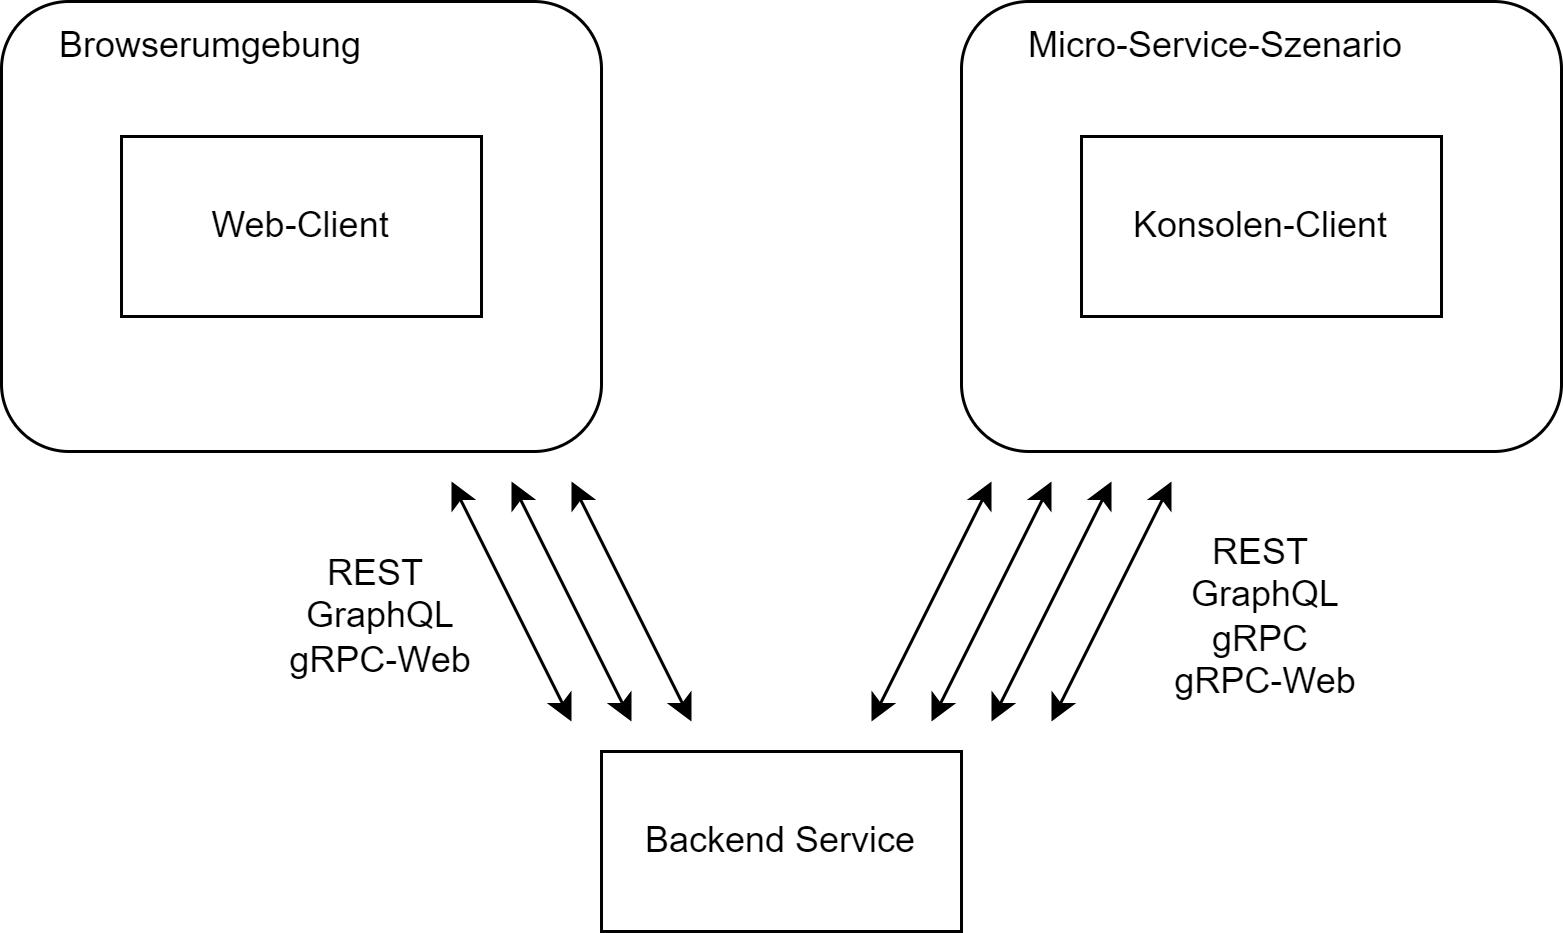
\includegraphics[width=0.9\textwidth]{images/Prototypschema.png}
	\caption{Schematischer Aufbau des Versuchs}
	\label{fig:backendservice}
\end{figure}

Die zwei verschiedenen Client-Typen können hierbei mit dem gemeinsamen Backend-System kommunizieren.

Der Schwerpunkt der Messungen liegt in folgenden Bereichen:

\begin{itemize}
	\item Vergleich einzelner und mehrfacher Requests
	\item Einfluss verschiedener Browser
	\item Unterschiede zwischen Microservice-Client und Browser-Client
\end{itemize}

\subsection*{Systemarchitektur:}

\subsubsection*{Front-End Clients:}
Der Versuchsaufbau beinhaltet zwei unabhängige Clients, die jeweils auf unterschiedliche Weise auf den Backend-Service zugreifen:
\begin{enumerate}
	\item Web-Client: die Übertragung findet dabei zwischen einem Browser und dem Back-End Service statt. Der Web-Client kann auf die REST, GraphQL und gRPC-Web API zugreifen.
	\item Konsolen Client: die Übertragung findet zwischen einer Microservice ähnlichen Konsolenanwendung und dem Back-End Service statt. Der Konsolen Client kann auf die REST, GraphQL, gRPC und gRPC-Web API zugreifen.
	
\end{enumerate}

\subsubsection*{Backend Service:}
Der Backend-Service stellt verschiedene Services zur Verfügung und kann von beiden Front-End Clients Anfragen entgegennehmen.
Die verschiedenen Services wurden so ausgewählt, dass die gesendeten Daten möglichst realitätsnahe Anwendungsfälle der Frontend-Backend Kommunikation abdecken.

\begin{figure}[htbp]
	\centering
	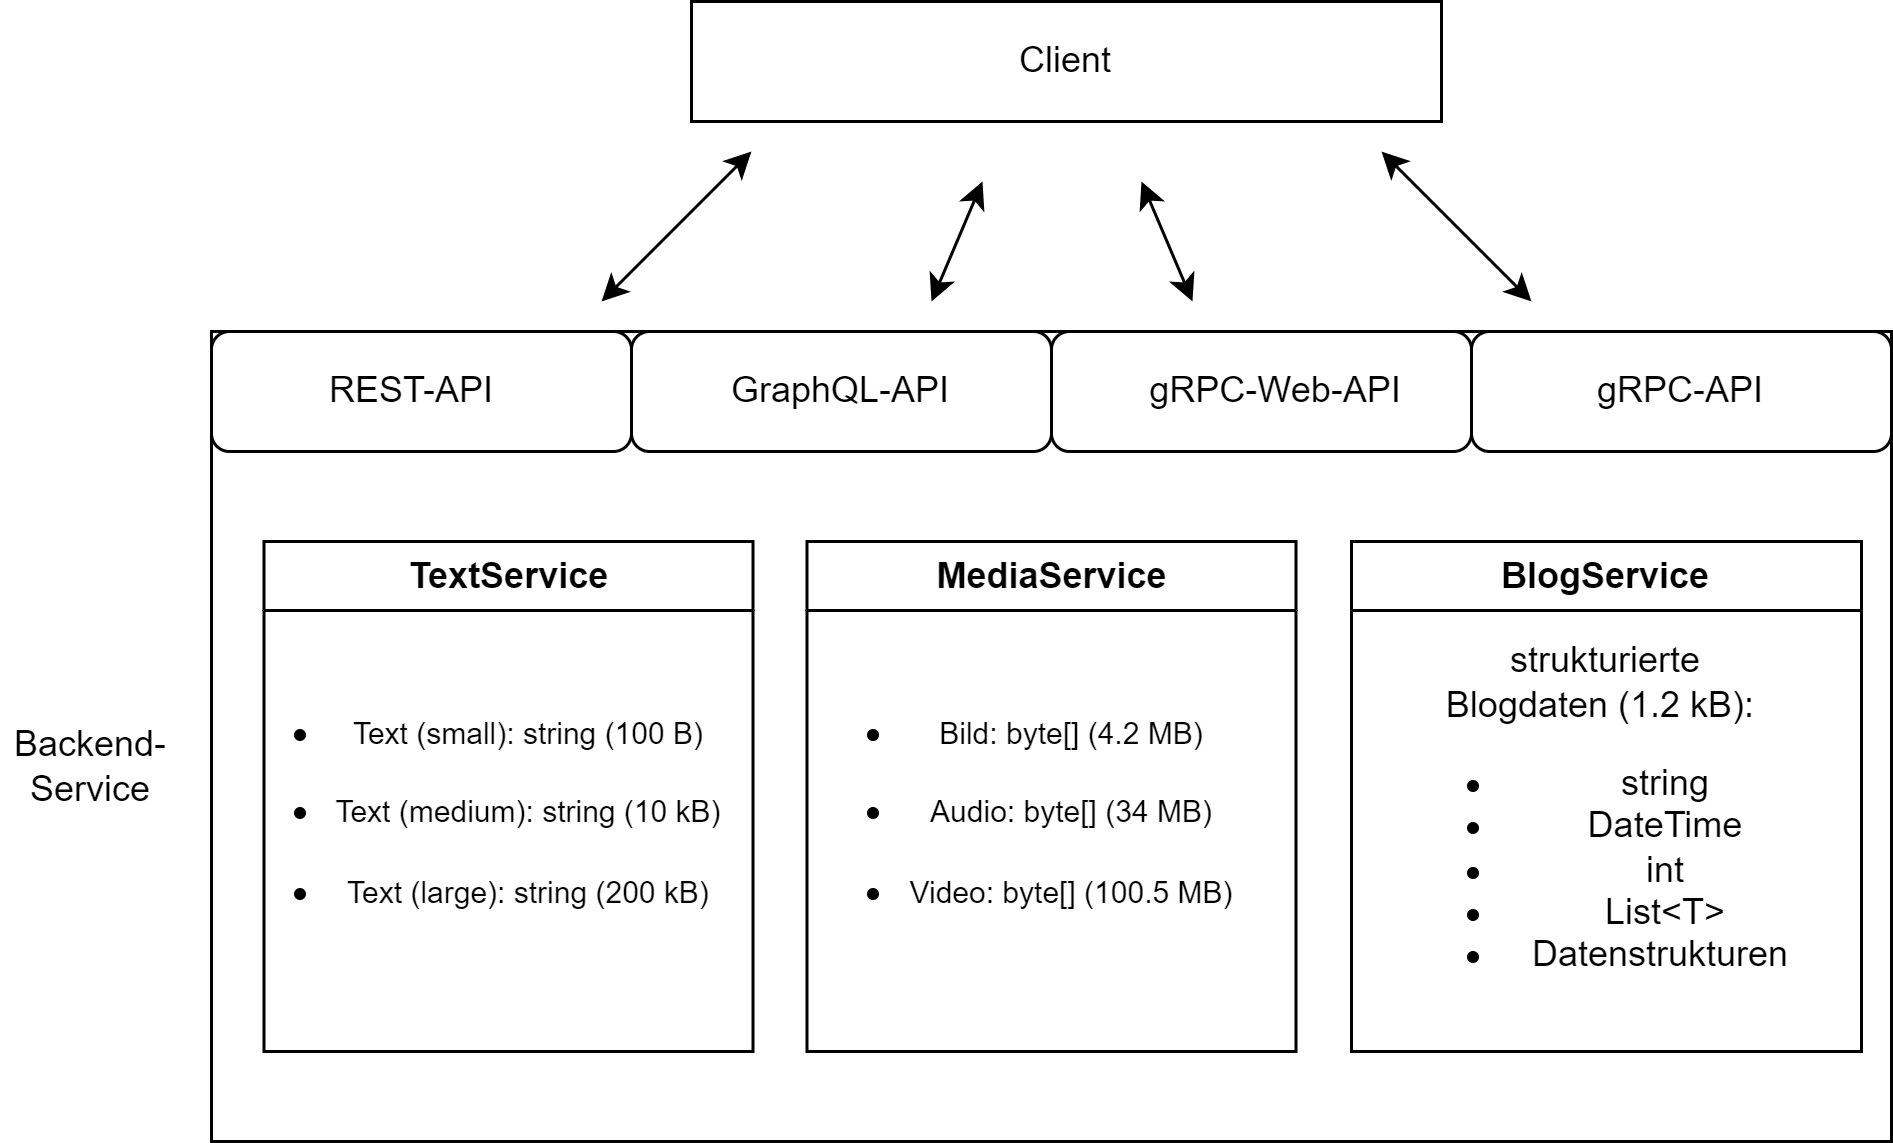
\includegraphics[width=0.85\textwidth]{images/BackendService.png}
	\caption{Schematischer Aufbau des Backend-Services mit Text-, Media- und Blog-Service}
	\label{fig:backendservice}
\end{figure}

Grundsätzlich, kann auf 3 verschiedene Services zugegriffen werden:

\begin{itemize}
	\item Text-Service: 
	Der Text-Service stellt einen Text im Datentyp „string“ zur Verfügung. Dabei können die Datengrößen 100 B, 10 kB und 200 kB abgefragt werden.
	
	\item Media-Service:
	Der Media-Service stellt Mediendaten zur Verfügung, die mittels eines byte[]-Arrays verschickt werden. Bei den Medien handelt es sich um ein Bild (4.2 MB), einer Audio-Datei (34 MB) und einem Video (100.5 MB). 
	
	\item Blog-Service: 
	Bei dem Blog-Service handelt es sich um einen 1.2 kB großen Datentypen, der verschachtelt andere Datentypen (int, string, DateTime, Listen, andere Datentypen) bereitstellt.
	
\end{itemize}

Alle Services wurden seperat mit den Technologien REST, GraphQL, gRPC und gRPC-Web implementiert und können somit von den jeweiligen Clients abgefragt und verglichen werden.

\subsection*{Testfälle:}
Zur Analyse der Client-Server Kommunikation wurden folgende Testfälle definiert, welche relevante Aspekte der Front-End Kommunikation abdecken und für einen adäquaten Vergleich der API-Technologien herangezogen werden können: 
\begin{itemize}
	\item \textbf{Einzelabfragen - Web-Client (1 Request):} Vergleich der Technologien bei beim senden eines einzelnen Requests. Dies wird jeweils bei jedem der definierten Services und für jede vorhandene Datengröße durchgeführt. Die Abfragen werden jeweils mit REST, GraphQL und gRPC-Web durchgeführt. Die Messungen zeigen Ergebnisse über Latenz und Performance.
	\item \textbf{Mehrfachabfragen - Web-Client ( 20 Requests ):} Analog zum Einzelrequest, wird der Versuch erneut mit Mehrfachabfragen durchgeführt, um zu sehen, wie gut die Technologien skalieren, Ressourcen nutzen und mehrere Requests effizient handhaben können.  
	\item \textbf{Unterschiede bei der Nutzung verschiedener Browser:} Um den Einfluss des Webbrowsers auf die Messungen des Web-Clients zu identifizieren, werden erneut Einzelrequests in verschiedenen Webbrowsern durchgeführt. Durch den Versuch wird festgestellt, ob eine Abhängigkeit des Browsers auf die Technologie besteht.
	\item \textbf{Einzelabfragen - Konsolen-Client (1 Request):} Analog zu den Einzelrequests des Web-Clients wird der Versuch erneut mit einem mircoservice-ähnlichen Konsolenclient durchgeführt. Hierbei wird jedoch auch abgesehen von REST, GraphQL und gRPC-Web die Latenz von gRPC gemessen. Durch den Versuch ist eine Gegenüberstellung der Response Zeiten zwischen den beiden Clients möglich.
\end{itemize}

Da es in Web Browsern nicht möglich ist "normales" gRPC zu verwenden, konnte diese Messung im Rahmen des Browser-Client-Versuchsaufbaus nicht durchgeführt werden. Um Messwerte zwischen gRPC und gRPC-Web zu vergleichen, und um zu sehen inwiefern sich die Performance zwischen Browser-Backend und Microservice-Backend unterscheiden, wurde der zweiter Versuchsaufbau mittels eines Konsolen-Clients durchgeführt.

\subsection*{Rahmenbedingungen}
Um einen fairen Vergleich herzustellen, wurden alle Requests ausschließlich mit dem HTTP/2.0 Protokoll durchgeführt und verschlüsselt mit HTTPS versendet. Bei der Response-Zeit handelt es sich jeweils um die End-zu-End-Latenz aus der Sicht des Nutzers. Es wird dabei die Zeit ab dem Absenden des Requestes bis zu dem Zeitpunkt, ab dem die Daten tatächlichen im Client fertig verarbeitet bereitstehen gemessen. Die Response Zeit beinhaltet also: 

\begin{enumerate}
	\item die Transportzeit über das Netzwerk:
	Zeit für den Hin- und Rückweg des Pakets durch das Netzwerk.
	
	\item Serverseitige-Verarbeitung:
	Die serverseitige Vearbeitung des Requests
	
	\item Antwortübertragung:
	Zeit für das Senden der Antwort(inklusive Header und Payload) zurück an den Client.
	
	\item Clientseitige Verarbeitung:
	die Verarbeitung des Responses, sodass die Daten tatsächlich im Client verwendet werden können. (JSON Parsing, Binär-Parser).
	
\end{enumerate}

\clearpage
\section{Implementierung}
Der Prototyp beinhaltet einen Backend-Service, einen Web-Client und einen Konsolen Client. Dieser Abschnitt befasst sich mit der Implementierung der jeweiligen Komponenten. 

Um die Vergleichbarkeit der jeweiligen API-Technologien zu erhöhen, wurden alle Clients und Services so minimalistisch wie möglich umgesetzt, da weitere Frameworks oder Logik die Datenverarbeitung beeinflussen, und somit die tatsächlichen Zeiten verzerren könnten.
Jeder Service liefert ausschließlich die für den Testfall angeforderten Daten. 
Die konkrete Implementierung ist auf GitHub verfügbar (siehe Quelle: \cite{muehlberger2025}).


Ziel dieses Abschnittes ist es die Architekturentscheidungen, Funktionsweisen sowie die technischen Aspekte darzustellen, auf Basis anschließend die Messungen durchgeführt werden.

\subsection{Backend-Service:}

Der Backend Service wurde modular und technisch getrennt umgesetzt, um die Technologien jeweils unabhängig voneinander vergleichen zu können. Die Implementierung basiert auf .NET 9, einer plattformunabhängigen Open-Source-Laufzeitumgebung von Microsoft, die für moderne Web- und Microservice-Anwendungen konzipiert ist.
Die Services stellen für jede der APIs dieselben Daten zur Verfügung und können folgendermaßen abgefragt werden:

\begin{itemize}
	\item REST: per HTTP-GET auf definierte Endpunkte.
	\item GraphQL: über einen einzigen Endpunkt, wobei der Client die benötigten Felder in der Query spezifiziert.
	\item gRPC und gRPC-Web: als typisierte RPC calls (Protobuf) 
\end{itemize}

\begin{table}[h]
	\centering
	\caption{Vergleich der API-Endpunkte}
	\label{tab:api-comparison}
	\renewcommand{\arraystretch}{1.2}
	\setlength{\tabcolsep}{4pt}
	\small
	\begin{tabularx}{\textwidth}{|l|>{\ttfamily}l|>{\ttfamily}l|>{\ttfamily}X|}
		\hline
		\textbf{Inhalt} & \textbf{REST-Endpunkt} & \textbf{gRPC-Methode} & \textbf{GraphQL-Abfrage} \\
		\hline
		Großer Text & GET /text/large & Text.GetLarge() & query \{ large \{ content \} \} \\
		\hline
		Video (MP4) & GET /media/video & Media.GetVideo() & query \{ video \} \\
		\hline
		Blogposts & GET /api/blog & Blog.GetAll() & query \{ posts \{ title, author... \} \} \\
		\hline
	\end{tabularx}
\end{table}




Die Struktur des Backend-Services gliedert sich in 4 eigenständige Projekte:

\begin{enumerate}
	\item Common:
	Das Common Projekt stellt die Testdaten zentral zur Verfügung. Damit die Testdaten bei einem Request nicht zuerst aus der Datei gelesen werden müssen, werden diese bei Programmstart einmal in den Arbeitsspeicher geladen. Zu diesem Zweck wurde ein API-Cache erstellt, der alle Text und Medienobjekte vorab einliest. Die Daten können dann zur Laufzeit direkt vom Cache abgefragt werden.
	
	Für die Testdaten wurden Datentypen die typischerweise an Web Clients gesendet werden ausgwählt und beinhalten:
	
	
	\begin{itemize}
		\item Texte in drei Größen: 100 B, 10 kB, 200 kB
		\item Medieninhalte: 4.2 MB Foto, 34 MB Audio-Datei, 100.5 MB Video-Datei
		\item Strukturierte Binärdaten: ein selbst definierter Datentyp mit verschachtelten Abschnitten, Metadaten, Zahlenblöcken und Autoreninformationen - 1.2 kB
	\end{itemize}
	\item RestAPI:
	Die REST API wurde mittels einem Controller Muster von ASP.NET Core implementiert und stellt 3 eigenständige Endpunkte zur Verfügung. Die Kommunikation erfolgt ausschließlich über HTTP GET.
	
	Die Controller sind wie folgt definiert:
	
	\begin{itemize}
		\item \textbf{TextController}: Stellt Textdaten in drei Größen zur Verfügung.\\
		\emph{Rückgabeformat}: \texttt{application/json}
		\item \textbf{MediaController}: Stellt ein Bild, eine Audiodatei und ein Video bereit.\\
		\emph{Rückgabeformat}: Binärdaten (\texttt{byte[]}) mit MIME-Type \texttt{image/jpeg}, \texttt{audio/wav}, \texttt{video/mp4}
		\item \textbf{BlogController}: Stellt einen vordefinierten Blogeintrag bereit.\\
		\emph{Rückgabeformat}: \texttt{application/json}
	\end{itemize}
	
	\item GraphQL-API:
	Die GraphQL-API wurde mittels des \texttt{.NET}-Frameworks \texttt{HotChocolate} implementiert.
	Als Einstiegspunkt wurde eine \texttt{Query}-Klasse definiert, welche für die verschiedenen Services (Text, Medien, Blog) jeweils erweitert wurde.
	
	Folgende Queries wurden definiert:
	\begin{itemize}
		\item \textbf{TextQuery}: Stellt die Felder \texttt{small}, \texttt{medium} und \texttt{large} bereit, welche jeweils Textinhalte als \texttt{string} zurückgeben.
		\item \textbf{MediaQuery}: Stellt die Felder \texttt{image}, \texttt{audio} und \texttt{video} bereit, welche in der GraphQL-Antwort Base64-kodiert übertragen werden.
		\item \textbf{BlogQuery}: Stellt das Feld \texttt{posts} zur Verfügung, welches die für den Blogpost definierten Daten enthält.
	\end{itemize}
	
	Alle Abfragen erfolgen über \texttt{HTTP~POST}-Anfragen an den Endpunkt \texttt{/graphql} und haben das Format \texttt{application/json}.
	
	\item GrpcWebAPI: 
	Die gRPC-Web-API basiert auf den definierten \texttt{.proto}-Dateien (\texttt{text.proto}, \texttt{media.proto}, \texttt{blog.proto}). In den Proto-Dateien wurden sowohl die \emph{Messages} und Datentypen der Testdaten als auch die \emph{Services}, mit denen auf die Messages zugegriffen werden kann, definiert. 
	
	Die Services implementieren folgende Methoden:
	\begin{itemize}
		\item \textbf{TextService}: Rückgabe der drei Textgrößen über die Methoden \texttt{GetSmall()}, \texttt{GetMedium()} und \texttt{GetLarge()}.\\
		\emph{Rückgabeformat}: \texttt{TextResponse}-Message mit einem \texttt{string}-Feld (\texttt{content}), serialisiert im Protocol-Buffers-Format.
		
		\item \textbf{MediaService}: Streaming von Binärdaten in 64\,kB-Chunks über die Methoden \texttt{GetImage()}, \texttt{GetAudio()} und \texttt{GetVideo()}. Anders als bei den anderen Services werden hier die Mediendateien nicht als vollständige Datei, sondern als 64\,kB-Chunks gestreamt. Da gRPC nicht dafür konzipiert wurde, große Dateien am Stück zu übertragen, ist dies die empfohlene Vorgehensweise für den Umgang mit großen Dateien. Bei REST und GraphQL hingegen wurde auf ein solches Streaming verzichtet, da entsprechende Mechanismen nicht nativ unterstützt werden.\\
		\emph{Rückgabeformat}: Server-Streaming von Chunk-Nachrichten (\texttt{bytes}-Feld), serialisiert als Protocol-Buffers-Stream über HTTP/2.
		
		\item \textbf{BlogService}: Rückgabe strukturierter Blogposts via \texttt{GetAll()}.\\
		\emph{Rückgabeformat}: \texttt{BlogPostsResponse} (Liste von \texttt{BlogPost}-Nachrichten), ebenfalls als Protocol Buffers kodiert.
	\end{itemize}
	
	Die API wurde so konfiguriert, dass sowohl normales gRPC als auch gRPC-Web verwendet werden kann. Die Implementierung für gRPC-Web wird mittels des Pakets \texttt{Grpc.AspNetCore.Web} bereitgestellt. Die Generierung der gRPC-eigenen Klassen erfolgte mittels \emph{gRPC Tools}. \emph{gRPC Tools} erstellt dabei bei jedem Build die im Proto-File definierten Klassen, die anschließend im Code verwendet werden können.
	
	 Tabelle~\ref{tab:technologienBackend} zeigt Libraries, Frameworks und Tools, sowie deren Versionen welche für die Implementierung des Backend-Services eingesetzt wurden.
	
	\begin{table}[h]
		\centering
		\caption{Verwendete Technologien Backend}
		\label{tab:technologienBackend}
		\begin{tabular}{lll}
			\hline
			\textbf{Komponente} & \textbf{Technologie/Tool} & \textbf{Version} \\
			\hline
			Backend-Framework & \texttt{.NET~SDK} & 9.0 \\
			REST API & \texttt{ASP.NET~Core~Web~API} & 9.0.5 \\
			GraphQL & \texttt{HotChocolate} & 15.1.5 \\
			gRPC & \texttt{Grpc.AspNetCore} & 2.71.0 \\
			gRPC-Web & \texttt{Grpc.AspNetCore.Web} & 2.71.0 \\
			Protobuf Tools & \texttt{Grpc.Tools} / \texttt{protoc} & 2.72.0 \\
			\hline
		\end{tabular}
	\end{table}
	
	\subsection{Web-Client:}
	Um die Messungen aus der Sicht eines Front-End-Clients durchzuführen, wurde ein Web-Client erstellt. Von der Anwendung aus, können die  Requests an die jeweiligen Services gesendet werden. Beim Senden eines Requests wird die End-zu-End Latenz im Client gemessen und anschließend mit der Payload grafisch angezeigt.  
	
	\begin{figure}[hbtp]
		\centering
		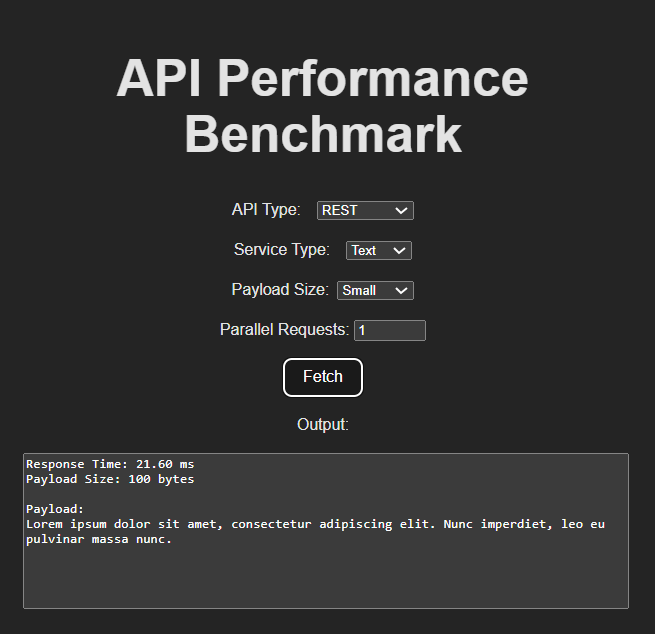
\includegraphics[width=0.8\textwidth]{images/frontendclient.png}
		\caption{Interface - Web-Client}
		\label{fig:frontendclient}
	\end{figure}
	
	 Die Implementierung wurde mit \texttt{React} und \texttt{TypeScript} durchgeführt und mithilfe von \texttt{Vite} gebündelt und lokal bereitgestellt.
	
	\subsubsection*{Architektur und Aufbau}
	Der Web-Client dient primär als Simulation eines realen Benutzerverhaltens einer Front-End-Anwendung. Über ein einfaches Interface kann ausgewählt werden:
	\begin{itemize}
		\item Gegen welche API-Schnittstelle (\texttt{REST}, \texttt{GraphQL}, \texttt{gRPC-Web}) ein Request ausgeführt werden soll
		\item Welche Datenart (Text, Medien, Blog) und welche Datenmenge übertragen werden soll
		\item Ob ein einzelner Request oder eine Mehrfachanfrage parallel durchgeführt werden soll
	\end{itemize}
	
	Sowohl bei REST als auch bei GraphQL wird im Frontend die browsernative \texttt{fetch}-API für die Kommunikation mit dem Backend verwendet.  
	Für die Kommunikation mit der gRPC-Web-Schnittstelle werden gRPC-Bibliotheken eingesetzt. Die Generierung der gRPC-Klassen erfolgt mittels der \texttt{ts-protoc-gen}-Bibliothek mit folgendem Befehl:
	
	\begin{verbatim}
		npx protoc --ts_out src/api/generated
		 --proto_path=src/proto src/proto/*.proto
	\end{verbatim}
	
	\subsubsection*{Clientseitige Datenverarbeitung}
	Nach erfolgreichem Empfang der Daten vom Server müssen die Daten vom Client verarbeitet werden, damit diese anschließend verwendet werden können. Abhängig vom ausgewählten API-Typ und der Datenmenge werden die Daten jeweils unterschiedlich verarbeitet. 
	
	\paragraph{Textdaten}
	\begin{itemize}
		\item Bei REST und GraphQL erfolgt das Parsen des gesendeten JSON mittels der nativen \texttt{fetch}-API.
		\item Bei gRPC-Web wird die Protobuf-Nachricht automatisch über die generierten TypeScript-Klassen des \texttt{protobuf-ts}-Plugins deserialisiert.
	\end{itemize}
	
	\paragraph{Mediendaten}
	
	Medieninhalte werden binär als \texttt{byte[]-Array} übertragen.
	\begin{itemize}
		\item Bei REST erfolgt der Empfang direkt als Blob über \texttt{response.blob()}.
		\item Bei GraphQL werden die Binärdaten Base64-kodiert als String im JSON-Response übertragen und im Client manuell dekodiert.
		\item Bei gRPC-Web werden die Binärdaten als Daten-Chunks gestreamt. Die Chunks werden im Client rekonstruiert.
	\end{itemize}
	
	\paragraph{Blogdaten}
	\begin{itemize}
		\item Bei REST und GraphQL werden JSON-Objekte mit verschachtelter Struktur geparst.
		\item Bei gRPC-Web erfolgt die Deserialisierung über generierte Protobuf-Klassen.
	\end{itemize}
	
		Tabelle~\ref{tab:frontend-tech} zeigt die Libraries, Frameworks und Tools, sowie deren Versionen welche für die Implementierung des Web-Clients eingesetzt wurden.
	
	\begin{table}[h]
		\centering
		\caption{Verwendete Frontend-Technologien}
	    \label{tab:frontend-tech}
		\begin{tabular}{lll}
			\hline
			\textbf{Komponente} & \textbf{Technologie/Tool} & \textbf{Version} \\
			\hline
			Frontend-Framework & \texttt{React} & 19.1.0 \\
			Bundler & \texttt{Vite} & 6.3.5 \\
			TypeScript Compiler & \texttt{TypeScript} & 5.8.3 \\
			REST & \texttt{fetch API} (Browser native) & (native) \\
			GraphQL Client & \texttt{fetch API} (Browser native) & (native) \\
			gRPC-Web Transport & \texttt{grpcweb-transport} & 2.11.0 \\
			Protobuf TS Plugin & \texttt{protobuf-ts} & 2.11.0 \\
			Protoc Codegen Plugin & \texttt{ts-protoc-gen} & 0.15.0 \\
			gRPC-Web Codegen & \texttt{protoc-gen-grpc-web} & 1.5.0 \\
			\hline
		\end{tabular}
	\end{table}
	
	\subsection{Konsolen-Client}
	 Um Messungen mit gRPC durchführen zu können wurde ein Konsolen-Clients implementiert. Dadurch können Response-Zeiten zwischen gRPC und gRPC-Web direkt miteinander verglichen werden. Außerdem kann aufgezeigt werden, wie sich gRPC, welches primär für Microservice-Architekturen erstellt wurde, im direkten Vergleich zu gRPC-Web verhält.
	
	Der Konsolen-Client kann alle unterstützten APIs (\texttt{REST}, \texttt{GraphQL}, \texttt{gRPC} und \texttt{gRPC-Web}) ansprechen und führt Messungen über ein textbasiertes Menüsystem durch.  
	Es werden nur Einzel-Requests unterstützt.
	
	\subsection*{Kommunikationsmechanismen}
	Die Kommunikation erfolgt jeweils über folgende Mechanismen:
	\begin{itemize}
		\item \textbf{REST}: per \texttt{HttpClient} mit JSON-Deserialisierung
		\item \textbf{GraphQL}: per \texttt{GraphQL.Client}-Bibliothek
		\item \textbf{gRPC}: über \texttt{Grpc.Net.Client} direkt als native gRPC-Kommunikation
		\item \textbf{gRPC-Web}: über \texttt{Grpc.Net.Client.Web} mittels spezieller Web-Handler, angepasst an das gRPC-Web-Protokoll
	\end{itemize}
	
	Die interne Verarbeitung wurde so implementiert, dass die Messungen die Response-Zeiten und anschließend das Parsen beinhalten.  
	Bei den Mediendaten findet auf Client-Seite keine weitere Verarbeitung des \texttt{byte[]}-Arrays statt, daher ist hier eine Gegenüberstellung zum Web-Client nicht sinnvoll.
	Tabelle~\ref{tab:console-tech} zeigt die Libraries, Frameworks und Tools, sowie deren Versionen welche für die Implementierung des Konsolen-Clients eingesetzt wurden.
	
	\begin{table}[h]
		\centering
		\caption{Verwendete Technologien des Konsolen-Clients}
		\label{tab:console-tech}
		\begin{tabular}{lll}
			\hline
			\textbf{Komponente} & \textbf{Technologie/Tool} & \textbf{Version} \\
			\hline
			Client-Framework & \texttt{.NET~SDK} & 9.0 \\
			GraphQL Client & \texttt{GraphQL.Client} & 6.1.0 \\
			GraphQL Client Serializer & \texttt{GraphQL.Client.Serializer.Newtonsoft} & 6.1.0 \\
			gRPC Client & \texttt{Grpc.Net.Client} & 2.71.0 \\
			gRPC-Web Client & \texttt{Grpc.Net.Client.Web} & 2.71.0 \\
			gRPC Code Generator & \texttt{Grpc.Tools} & 2.72.0 \\
			\hline
		\end{tabular}
	\end{table}
	
\end{enumerate}
\section{Spezifikationen des Testsystems}
Um die Messergebnisse korrekt und vergleichbar einordnen zu können, ist es notwendig darzustellen, unter welchen technischen Rahmenbedingungen die jeweiligen Messungen durchgeführt wurden. Da die Leistungsfähigkeit der Hardware sowie die Softwareversionen die Messzeiten beeinflussen können.
Für die Messungen wurde folgendes Testgerät verwendet:  
Lenovo ThinkPad X1 Carbon der 10.\ Generation (Modellbezeichnung: 21CB)
\paragraph{Hardwarekonfiguration}
\begin{itemize}
	\item \textbf{Prozessor (CPU)}: 12th Gen Intel\textsuperscript{\textregistered} Core\texttrademark{} i5-1245U, 1600\,MHz, 10~Kerne
	\item \textbf{Arbeitsspeicher (RAM)}: 16\,GB LPDDR5, 5200\,MT/s
	\item \textbf{Massenspeicher (SSD)}: 512\,GB NVMe SSD
\end{itemize}

\paragraph{Betriebssystem:}
Microsoft Windows 11 Pro (Version: 10.0.26100, Build 26100)

\clearpage
\section{Messung}
Ziel der Messungen ist es, die End-zu-End-Latenz und Performance bei der Datenübertragung zwischen Frontend und Backend zu quantifizieren und somit die im theoretischen Teil beschriebenen Eigenschaften der verschiedenen API-Technologien mit einem praktischem Anwendungsfall zu vergleichen.  
Die Responsezeiten beschreiben die tatsächliche Zeit, bis die jeweiligen Daten im Client bereitstehen (Datenübertragung und Parsing). Dabei wurden unterschiedliche Datenarten verwendet, die häufig in der Frontend-zu-Backend-Kommunikation zum Einsatz kommen.  

Untersucht wurde die Response-Zeit von Einzel-Requests, Mehrfachabfragen (20 parallele Requests) und browserabhängige Unterschiede in einem Web-Client. Zusätzlich wurden alle Technologien (REST, GraphQl, gRPC-Web und gRPC) im Konsolen-Client getestet, um Unterschiede zwischen browserbasierter und microservice-orientierter Kommunikation sichtbar zu machen und Unterschiede zwischen gRPC und gRPC-Web zu ermitteln.

Für den Vergleich der Messwerte wurde der gerundete arithmetische Mittelwert herangezogen, sofern die Abweichung zum Median nicht zu groß war und damit ausgeschlossen werden konnte, dass der Mittelwert durch Ausreißer verzerrt wurde. Zur besseren grafischen Darstellung der Daten wurde die y-Achse der Diagramme logarithmisch skaliert.

Die Messungen wurden ausschließlich lokal auf localhost durchgeführt. Dadurch können zusätzliche Einflüsse wie Paketverlust, Routing-Latenz oder Bandbreitenschwankungen, die bei realen Bedingungen auftreten würden, ausgeschlossen worden. Ziel der Messungen war es, tatsächliche Unterschiede zwischen den API Technologien (gRPC, gRPC-Web, REST, GraphQL) unter optimalen Bedingungen und reproduzierbar zu ermitteln.
Der Fokus wurde ausschließlich auf den Vergleich der Kommunikationsprotokolle und deren Verarbeitung gelegt.

Die Ergebnisse der Messungen liefern eine Grundlage zur Beantwortung der Forschungsfragen, inwiefern sich die Schnittstellentechnologien hinsichtlich der Effizienz und Eignung für typische Frontend-Szenarien unterscheiden.  
Die nachfolgenden Abschnitte stellen die gemessenen Daten dar und geben einen direkten Vergleich der Technologien.

\clearpage
\subsection{Web-Client (Einzel-Request)}

Bei der Messung der End-zu-End Latenz ergaben sich zwischen den einzelnen Technologien erhebliche Unterschiede. 
Für eine sinnvolle Auswertung der Daten, wurden jeweils 30 Requests unabhängig voneinander durchgeführt die Durschnittszeiten und der Median aus den gemessenen Daten ermittelt. 

\begin{table}[h]
	\centering
	\caption{Chrome-Client – Einzel-Requests: Durchschnitt und Median (Antwortzeit in ms)}
	\label{tab:chrome-single-avg}
	\renewcommand{\arraystretch}{1.1}
	\begin{tabular}{|l|l|l|r|r|}
		\hline
		\textbf{Technologie} & \textbf{Service} & \textbf{Datentyp} & \textbf{AVG} & \textbf{MEDIAN} \\
		\hline
		REST & Text  & small text  & 8.6 & 8.7 \\
		&       & medium text & 9.0 & 8.8 \\
		&       & large text  & 13.2 & 12.9 \\
		& Media & Foto        & 36.1 & 36.5 \\
		&       & Audio       & 148.9 & 151.6 \\
		&       & Video       & 365.0 & 353.6 \\
		& Blog  & -           & 8.6 & 8.2 \\
		\hline
		GraphQL & Text  & small text  & 7.6 & 7.4 \\
		&       & medium text & 7.7 & 7.6 \\
		&       & large text  & 10.1 & 9.8 \\
		& Media & Foto        & 511.7 & 490.5 \\
		&       & Audio       & 5896.9 & 5658.3 \\
		&       & Video       & - & - \\
		& Blog  & -           & 7.6 & 7.2 \\
		\hline
		gRPC-Web & Text  & small text  & 7.5 & 7.5 \\
		&       & medium text & 8.4 & 8.3 \\
		&       & large text  & 18.8 & 18.8 \\
		& Media & Foto        & 182.0 & 162.6 \\
		&       & Audio       & 2372.5 & 2355.0 \\
		&       & Video       & - & - \\
		& Blog  & -           & 7.9 & 7.8 \\
		\hline
	\end{tabular}
\end{table}

\clearpage

\begin{figure}[htbp]
	\centering
	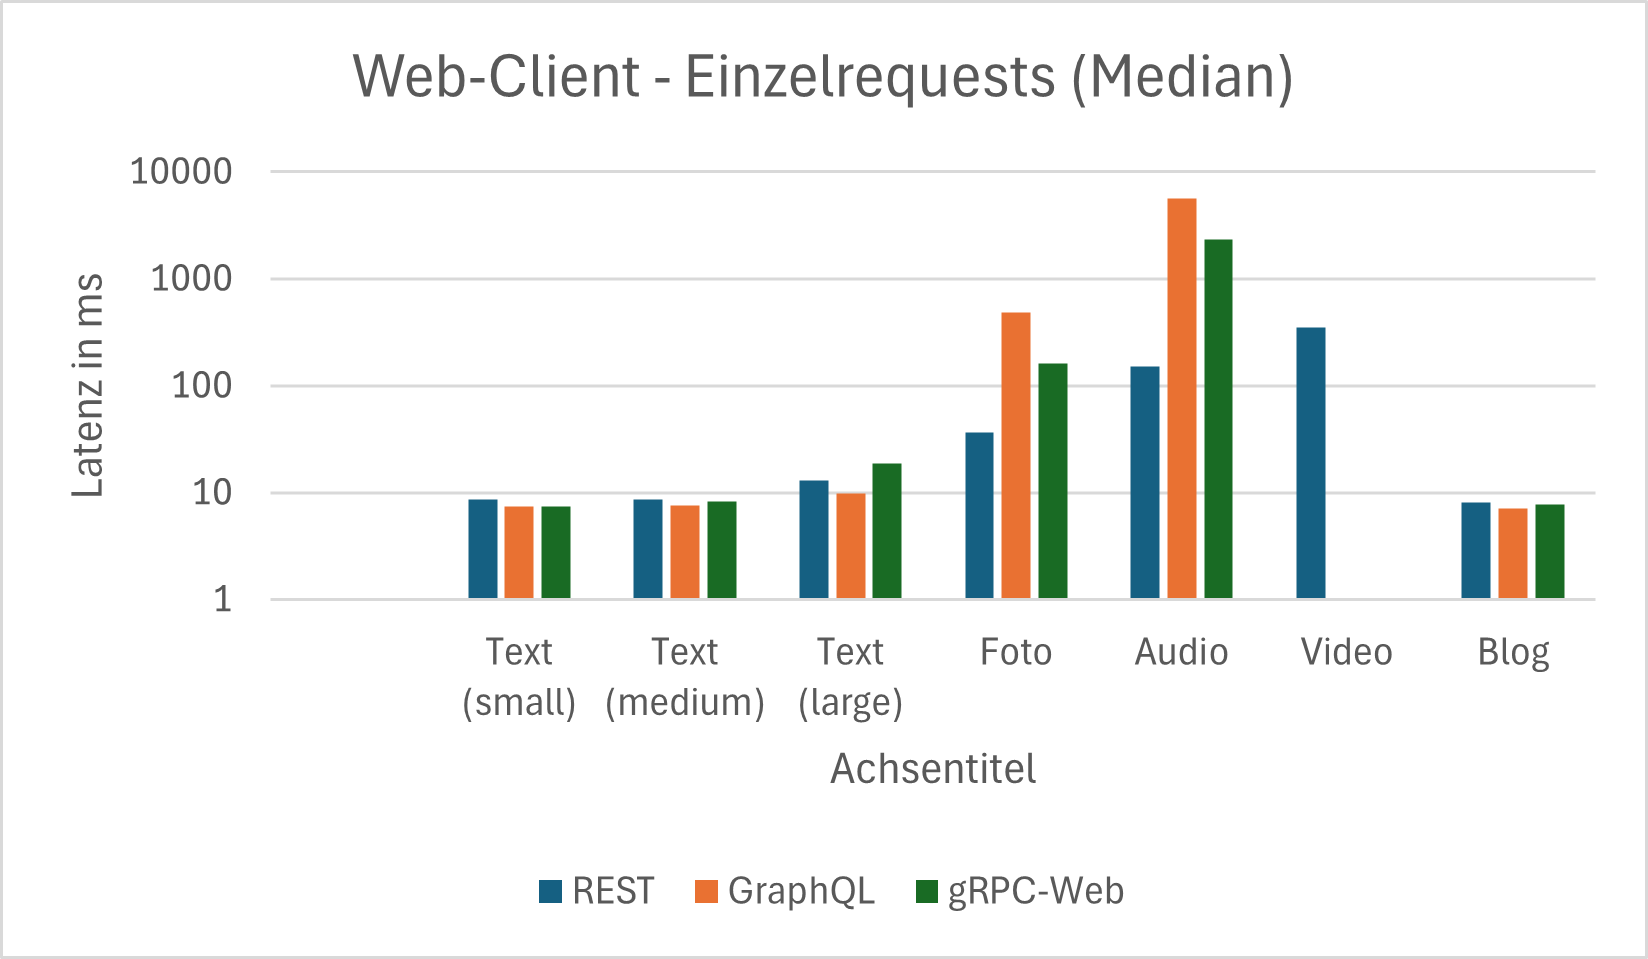
\includegraphics[width=0.9\textwidth]{images/Webclient.png}
	\caption{Web-Client - Einzel-Request: End-to-End-Latenz (Median) je Datentyp und Technologie [ms]}
	\label{fig:webclient-single-median}
\end{figure}

\textbf{Text-Service:}  
Es ist zu erkennen, dass kleinere Textdaten (100 B-10 kB) von allen Schnittstellen relativ schnell verarbeitet werden konnten. gRPC Web und GraphQL weisen hierbei jedoch die geringsten Antwortzeiten (7.5-8.5 ms) auf, REST benötigte ungefähr 8-9 ms für kleinere Textdaten. Bei größeren Textmengen (200 kB) steigt die Latenz erwartungsgemäß bei allen Technologien etwas an, wobei diese bei GraphQl mit 10 ms und REST mit 13 ms deutlich schneller als bei gRPC Web (19 ms) bereitstehen. 

\textbf{Media-Service:}  
Besonders auffällig ist der Leistungsunterschied bei der Übertragung von Mediendaten.
Hierbei war entgegen der theortischen Erwartungen REST die schnellste Technologie für alle Medienarten. Für Bilder ( 4MB) lag dabei die mittlere Antwortzeit bei 36 ms, deutlich vor gRPC ( 182 ms ) und GraqhQL ( 511 ms ).
Ähnliches Verhalten zeigte sich bei der Übertragung von Audiodateien (34 MB), hierbei wurde mit REST eine mittlere Antwortzeit von 149 ms gemessen, mit deutlichem Abstand gefolgt von gRPC ( 2372 mms) und GraphQL ( 5897  ms ).
Bei der Übertagung von Videodaten (100 MB ) konnte in Chrome keine vergleichbare Messung der Antwortzeiten durchgeführt werden. Die Übertragung war nur über die REST-API erfolgreich. Es ergab sich dabei eine durchschnittliche Antwortzeit von 365 ms. Wegen großer Ladezeit bzw. Instabilitäten des Clients konnten für GraphQL und gRPC-Web keine Daten gemessen werden. 


\textbf{Blog-Service:}  
Bei der Messung der Blogdaten, konnten geringe Unterschiede in den Abfragezeiten zwischen den Technologien identifiziert werden. GraphQL war hierbei mit einer mittleren Latenz von 7.6 ms leicht schneller als gRPC-Web ( 7.9 ms) und REST (8.6 ms).

\subsection{{Web-Client (Parallele-Requests)}}
Bei der Durchführung von 20 parallelen Requests wurden jeweils pro API und Service 30 Messwerte (Ausnahme: Media-Service) gemessen und anschließend der Durchschnittswert und Median berechnet. Es zeigten sich erwartungsgemäß höhere Latenzen gegenüber der Einzelabfragen. 

\begin{table}[h]
	\centering
	\caption{Chrome-Client – 20 parallele Requests: Durchschnitt und Median (Antwortzeit in ms)}
	\label{tab:chrome-20req}
	\renewcommand{\arraystretch}{1.1}
	\begin{tabular}{|l|l|l|r|r|}
		\hline
		\textbf{Technologie} & \textbf{Service} & \textbf{Datentyp} & \textbf{AVG} & \textbf{Median} \\
		\hline
		REST & Text  & small text  & 45.5 & 44.0 \\
		&       & medium text & 61.9 & 62.0 \\
		&       & large text  & 92.1 & 93.6 \\
		& Media & Foto        & 385.8 & 384.6 \\
		&       & Audio       & 2420.1 & 2393.4 \\
		&       & Video       & - & - \\
		& Blog  & -           & 53.0 & 48.3 \\
		\hline
		GraphQL & Text  & small text  & 31.4 & 29.0 \\
		&       & medium text & 35.4 & 33.4 \\
		&       & large text  & 71.1 & 68.7 \\
		& Media & Foto        & 16159.6 & 15745.7 \\
		&       & Audio       & - & - \\
		&       & Video       & - & - \\
		& Blog  & -           & 34.6 & 33.0 \\
		\hline
		gRPC-Web & Text  & small text  & 33.4 & 32.1 \\
		&       & medium text & 43.5 & 40.9 \\
		&       & large text  & 145.3 & 145.4 \\
		& Media & Foto        & 5736.2 & 5682.4 \\
		&       & Audio       & 126026.5 & 107938.0 \\
		&       & Video       & - & - \\
		& Blog  & -           & 34.5 & 31.3 \\
		\hline
	\end{tabular}
\end{table}
\clearpage

\begin{figure}[htbp]
	\centering
	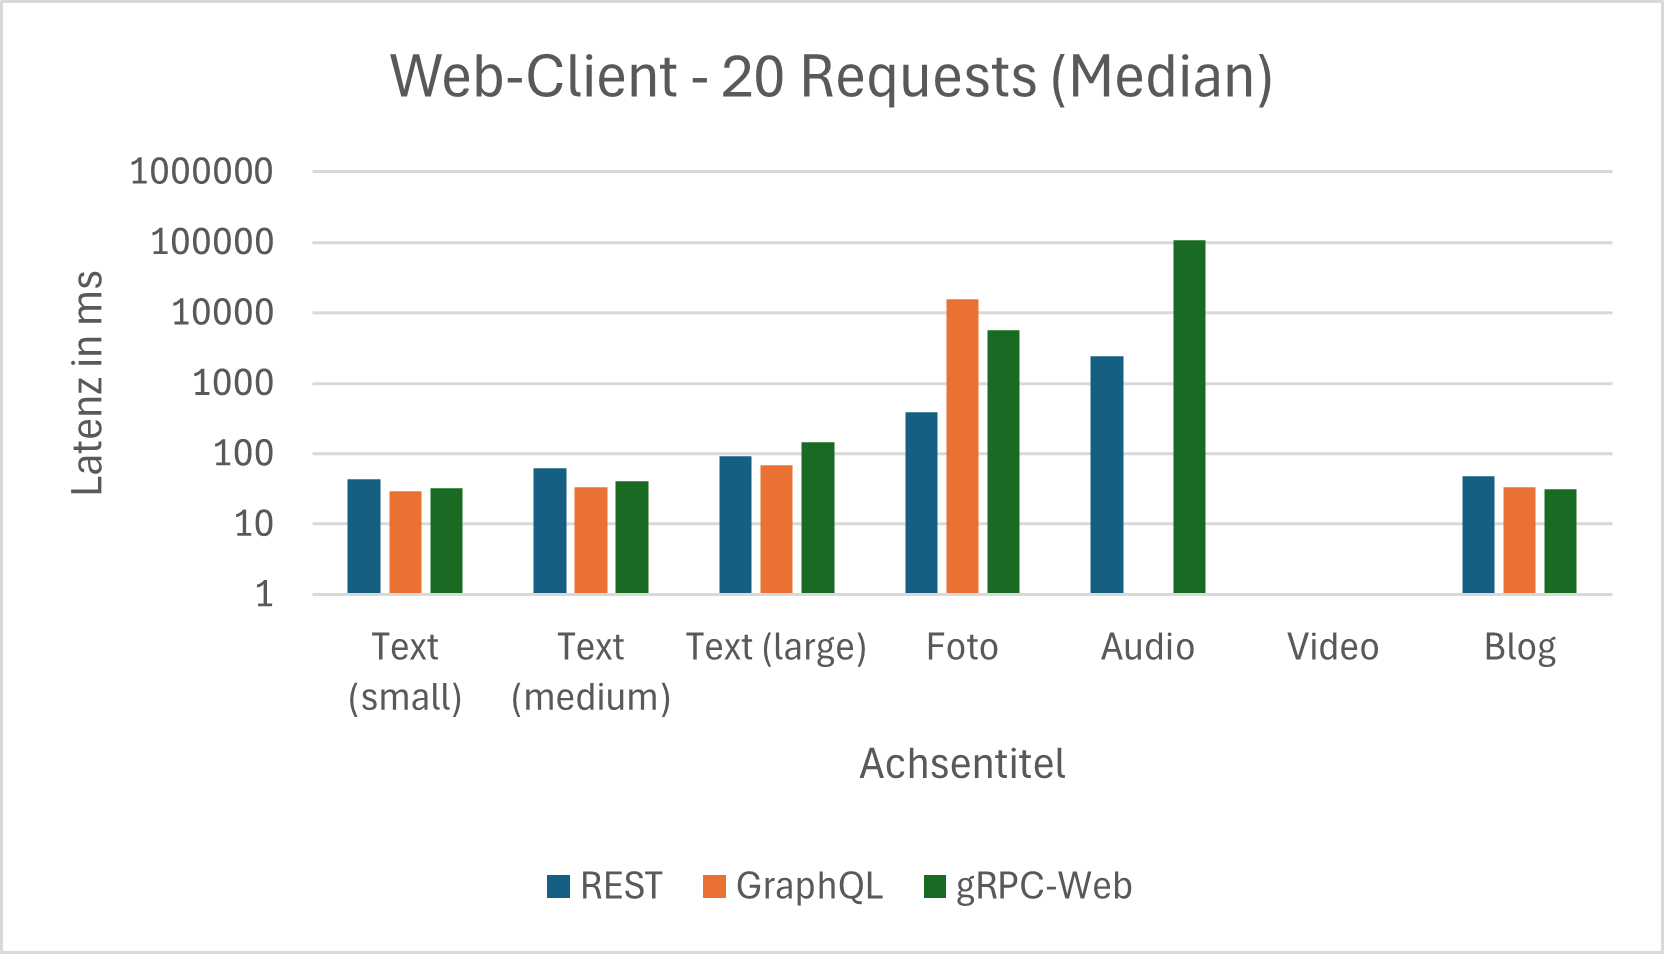
\includegraphics[width=0.9\textwidth]{images/Parallelrequests.png}
	\caption{Web-Client - 20 parallele Requests: End-to-End-Latenz (Median) je Datentyp und Technologie [ms]}
	\label{fig:webclient-20req-median}
\end{figure}

\textbf{Text-Service:}  
Während kleinere Textdaten noch performant verarbeitet werden können, nehmen die Unterschiede bei größeren Lasten stärker zu. Bei sehr kleinen Textdaten von 100 B sind gRPC-Web und GraphQL jeweils mit einer Antwortzeit von 31ms (GraphQL) und 33 ms (gRPC-Web) gleichauf, bei 10 kB ist graphQL mit 35 ms ungefähr 9 ms schneller als gRPC-Web mit 44 ms. Je größer die Daten werden, desto langsamer wird gRPC-Web. REST benötigte bei den kleineren Lasten 46 ms für 100 B und 62 ms für 10 kB. Auch bei größeren Textdaten ist GraphQL mit 71 ms am schnellsten, gefolgt von REST mit 92 ms und gRPC-Web mit 145 ms. 

\textbf{Media-Service:}  
Bei der Verarbeitung von Medien kam es wie bereits durch die einzelabfragen erwartet zu größeren Unterschieden. REST schnitt auch hier mit 386 ms für Fotos und 2420 ms für Audiodaten am besten ab. Gefolgt von gRPC-Web mit 5736 ms für das Foto und 126026 ms für die Audiodatei. Bei GraphQL dauerte der Request für die Fotodaten 16159 ms.
Für Video- bzw. Audiodateien (GraphQL) wurden aufgrund des bereits bei den Einzelabfragen instabilen Ladeverhaltens keine weiteren Messungen durchgeführt.


\textbf{Blog-Service:}  
Bei den Abfragen der Blogdaten lagen die Antwortzeiten aller Technologien im zweistelligen ms Bereich. Ähnlich wie bei kleineren Textdaten, sind gRPC-Web und GraphQL mit jeweis 35 ms gleichauf, gefolgt von REST mit 53 ms.

\clearpage
\subsection{Browser-Vergleich}
Derselbe Versuch mit Einzel-Requests wurde anschließend in zwei weiteren Web Browsern durchgeführt, um festzustellen, ob es bei der Performance der APIs eine Abhängigkeit vom Webbrowser gibt. 
Bei der Messung wurden jeweils 10 Requests pro Technologie und Service durchgeführt und daraus der Durchschnitt und der Median ermittelt.

	\begin{table}[h]
		\centering
		\caption{Vergleich WebClient (1 Request) – Chrome, Firefox, Edge (AVG in ms)}
		\label{tab:browser-comparison-1req}
		\renewcommand{\arraystretch}{1.2}
		\begin{tabular}{|l|l|l|r|r|r|}
			\hline
			\textbf{Technologie} & \textbf{Service} & \textbf{Datentyp} & \textbf{Chrome} & \textbf{Firefox} & \textbf{Edge} \\
			\hline
			REST & Text  & small text  & 8.6   & 8.5   & 4.84 \\
			&       & medium text & 9.0   & 9.3   & 6.31 \\
			&       & large text  & 13.2  & 11.4  & 9.5  \\
			& Media & Foto        & 36.1  & 54.4  & 36.3 \\
			&       & Audio       & 148.9 & 248.7 & 144.9 \\
			&       & Video       & 365.0 & 676.4 & 422.8 \\
			& Blog  & -           & 8.6   & 6.7   & 7.9  \\
			\hline
			GraphQL & Text  & small text  & 7.6   & 9.4   & 5.61 \\
			&       & medium text & 7.7   & 11.1  & 5.68 \\
			&       & large text  & 10.1  & 15.8  & 8.21 \\
			& Media & Foto        & 511.7 & 1743.4 & 402.8 \\
			&       & Audio       & 5896.9 & 13253.3 & 6442.1 \\
			&       & Video       & -     & 90091  & - \\
			& Blog  & -           & 7.6   & 9.6   & 5.6 \\
			\hline
			gRPC-Web & Text  & small text  & 7.5   & 9.4   & 5.5 \\
			&       & medium text & 8.4   & 9.4   & 5.7 \\
			&       & large text  & 18.8  & 24.2  & 20.3 \\
			& Media & Foto        & 182.0 & 248.1 & 186.4 \\
			&       & Audio       & 2372.5 & 2455.6 & 2744.9 \\
			&       & Video       & -     & 8984.8 & 7984.6 \\
			& Blog  & -           & 7.9   & 8.0   & 5.2 \\
			\hline
		\end{tabular}
	\end{table}

\clearpage

\begin{figure}[htbp]
	\centering
	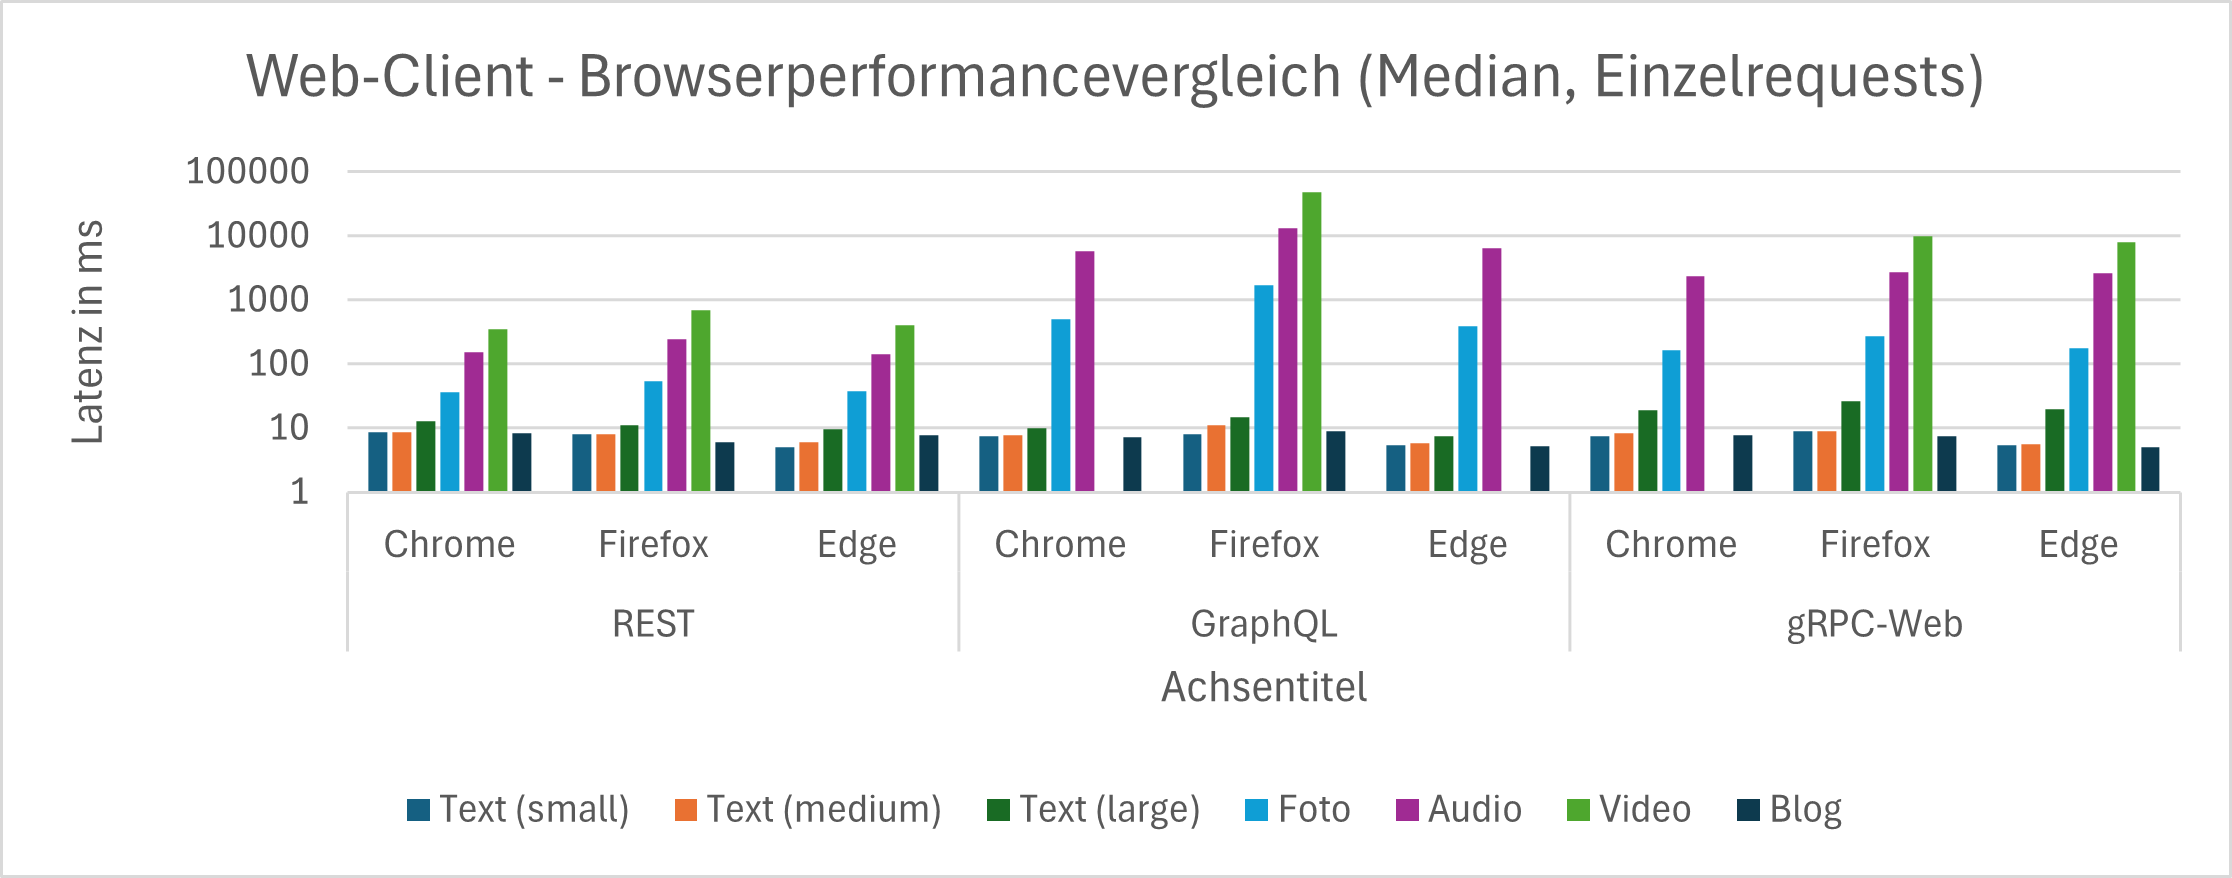
\includegraphics[width=0.9\textwidth]{images/Browserperformance.png}
	\caption{Web-Client - Browser-Vergleich (Einzel-Request): End-to-End-Latenz (Median) je Datentyp und Technologie [ms]}
	\label{fig:webclient-browser-comparison}
\end{figure}

\textbf{Textdaten:}  
Bei den Messungen reagierte Edge in allen Schnittstellen mit den niedrigsten Antwortzeiten, dabei konnten bei allen drei API-Architekturen deutliche Unterschiede gemessen werden. Für kleinere Textdaten (100 B bis 10 kB) benötigten Chrome und Firefox bei REST 8.5-9.5 ms während Edge nur 4.8 und 6.3 ms benötigte. Ähnlich ist das Verhalten bei GraphQL und gRPC-Web wobei Chrome bei diesen Architekturen deutlich schneller als Firefox ist. Auch bei größeren Textmengen blieg Edge bei allen Technologien am performantesten. Bei GraphQL und gRPC-Web war Chrome wieder schneller als Firefox. Bei dem REST Service war Firefox jedoch mit 11 ms schneller als Chrome (13 ms).


\textbf{Medieninhalte (Foto, Audio, Video)}  
Beim Senden von Mediendaten hatten Chrome und Edge im Gegensatz zu Firefox eine ähnliche Performance. Bei REST und gRPC-Web konnten Edge und Chrome die kürzesten Antwortzeiten für Fotos (36 ms) und Audiodateien (ungefähr 150 ms)  liefern. Bei Firefox lagen diese bei REST bei 54 ms und 249 ms bzw. bei gRPC-Web bei 250 ms und 2455 ms.

Bei dem Senden von Videodaten war Chrome am performantesten. Hier hatte REST eine Antwortzeit von 365 ms, Edge 423 ms und Firefox 676 ms. Im Gegensatz zu Chrome, konnte das Video in Firefox mit gRPC-Web (8984 ms) und Edge ( 7984 ms) dargestellt werden. In Firefox war sogar ein laden mit GraphQL möglich (90091 ms), auch wenn dies sehr lange dauerte.


\textbf{Blogdaten:}  
Wie bei Textdaten ist Edge auch bei dem Senden von Blogdaten in allen Kategorien am schnellsten. Während Chrome und Firefox bei gRPC-Web mit 8 ms gleich schnell sind, ist Firefox bei REST mit 7 ms zu 9 ms und Chrome bei GraphQL mit 8 ms zu 10 ms schneller als der jeweils andere Browser.


\clearpage
\subsection{Konsolen-Client (Einzel-Request)}
Um die Kommunikationsleistung der einzelnen Technologien ohne Einfluss eines Browers aufzuzeigen, und um einen direkten Performancevergleich zwischen gRPC und gRPC-Web zu ermitteln wurden ebenfalls Messungen in der Kommunikation innerhalb einer Microservice basierten Architektur untersucht. Wie erwartet sind die Messewerte in dieser Messung zum größten Teil deutlich besser als zwischen Web-Client und Backend Service.  

\begin{table}[h]
	\centering
	\caption{Konsole – 1 Request: Durchschnitt und Median (Antwortzeit in ms)}
	\label{tab:console-1req}
	\renewcommand{\arraystretch}{1.1}
	\begin{tabular}{|l|l|l|r|r|}
		\hline
		\textbf{Technologie} & \textbf{Service} & \textbf{Datentyp} & \textbf{AVG} & \textbf{Median} \\
		\hline
		REST & Text  & small text  & 2.3 & 2.0 \\
		&       & medium text & 2.1 & 2.0 \\
		&       & large text  & 6.4 & 7.0 \\
		& Media & Foto        & 45.9 & 41.5 \\
		&       & Audio       & 250.4 & 249.5 \\
		&       & Video       & 540.2 & 515.0 \\
		& Blog  & -           & 1.0 & 1.0 \\
		\hline
		GraphQL & Text  & small text  & 2.3 & 2.0 \\
		&       & medium text & 2.2 & 2.0 \\
		&       & large text  & 5.5 & 5.0 \\
		& Media & Foto        & 5716.2 & 5742.0 \\
		&       & Audio       & - & - \\
		&       & Video       & - & - \\
		& Blog  & -           & 2.4 & 2.0 \\
		\hline
		gRPC-Web & Text  & small text  & 2.2 & 2.0 \\
		&       & medium text & 2.8 & 3.0 \\
		&       & large text  & 6.8 & 7.0 \\
		& Media & Foto        & 51.3 & 53.0 \\
		&       & Audio       & 251.4 & 248.0 \\
		&       & Video       & 705.1 & 717.5 \\
		& Blog  & -           & 2.9 & 3.0 \\
		\hline
		gRPC & Text  & small text  & 1.2 & 1.0 \\
		&       & medium text & 1.5 & 1.5 \\
		&       & large text  & 4.1 & 4.0 \\
		& Media & Foto        & 42.7 & 41.0 \\
		&       & Audio       & 252.1 & 249.0 \\
		&       & Video       & 610.0 & 615.0 \\
		& Blog  & -           & 1.1 & 1.0 \\
		\hline
	\end{tabular}
\end{table}

\clearpage

\begin{figure}[htbp]
	\centering
	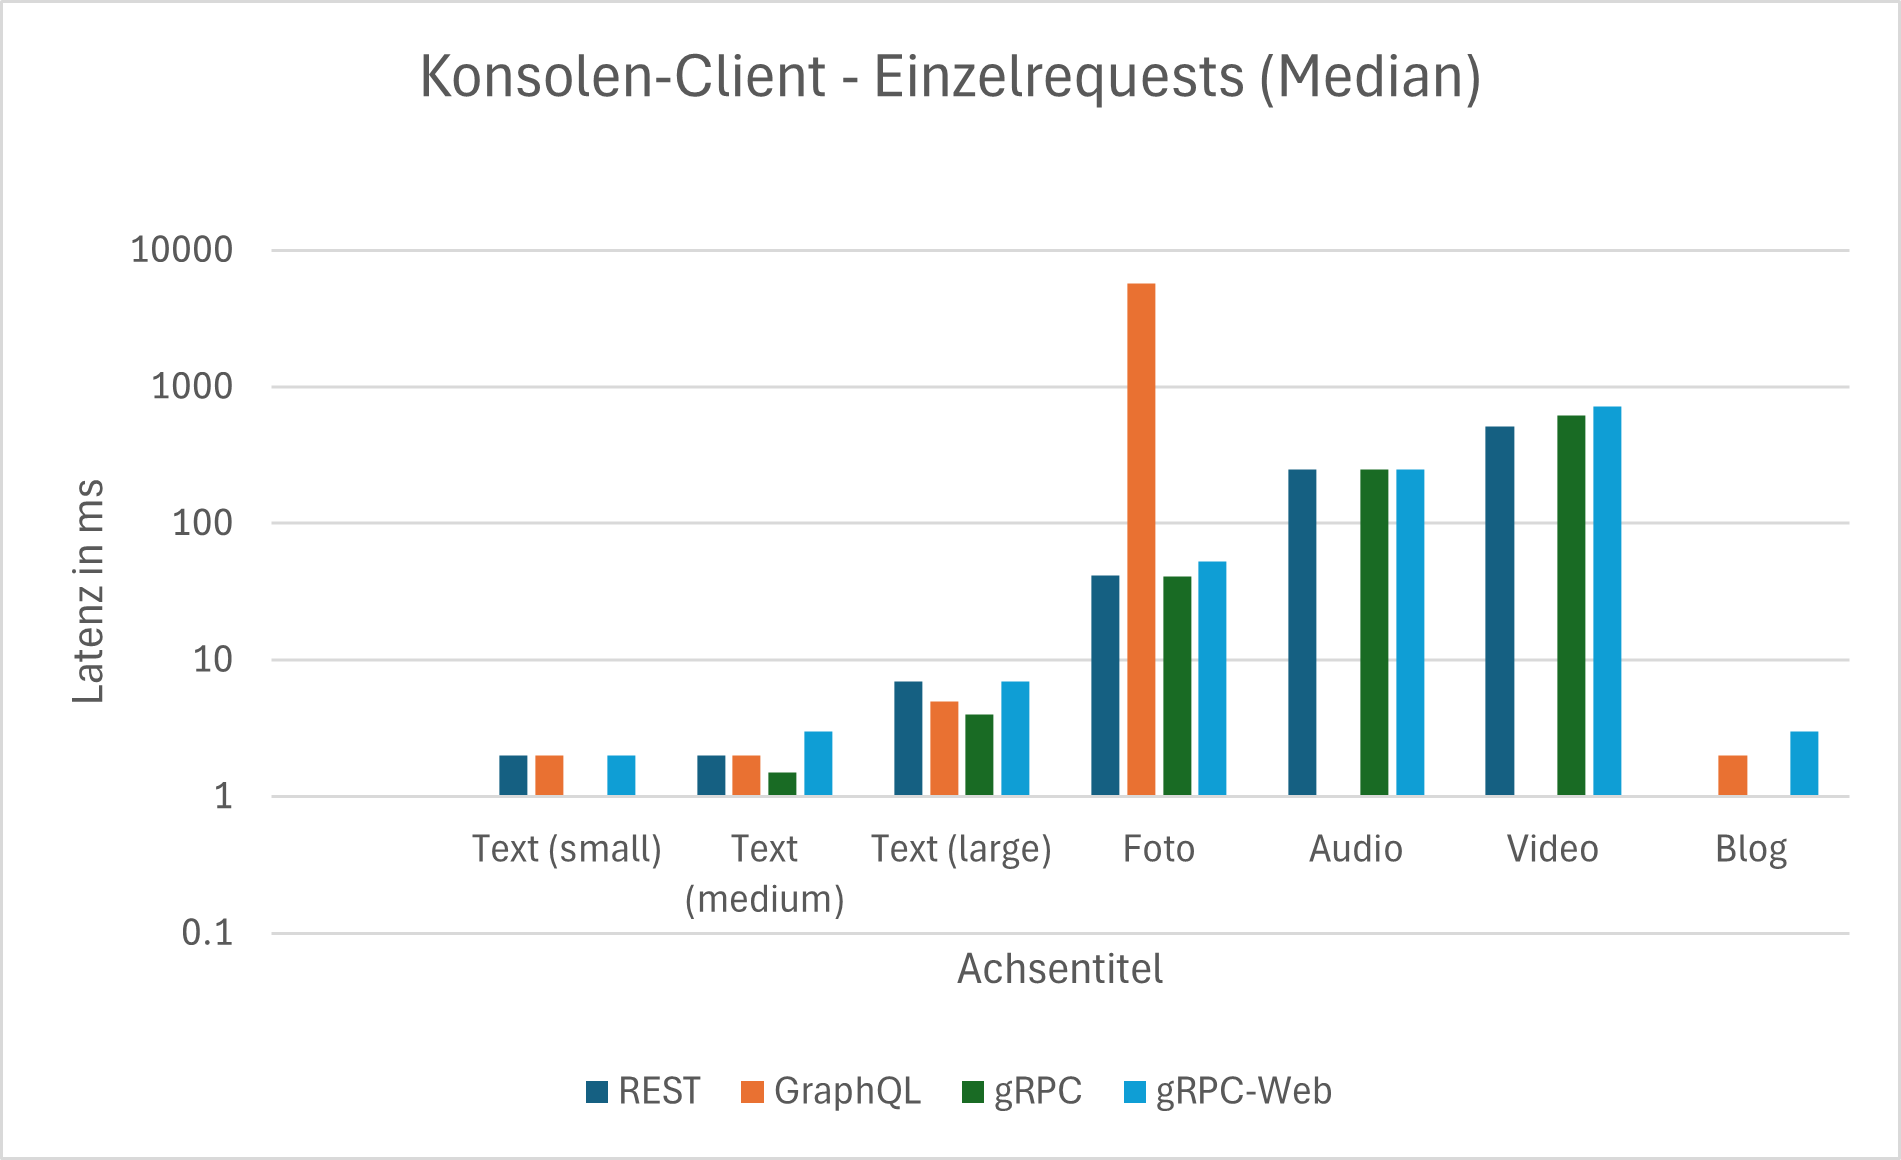
\includegraphics[width=0.9\textwidth]{images/Konsolenclient.png}
	\caption{Konsolen-Client - Einzel-Request: End-to-End-Latenz (Median) je Datentyp und Technologie [ms]}
	\label{fig:console-client-1req}
\end{figure}

\textbf{Text-Service:}  
Alle Technologien zeigten bei kleinen und mittleren Textdaten im Konsolen-Client sehr geringe Antwortzeiten. gRPC hatte hier jedoch eindeutlig die schnellste Response Zeit mit nur 1.2 für 100 B und 1.5 ms für 10 kB. REST, GraphQL und gRPC-Web haben ungefähr die selbe Reponse-Zeit von 2 ms für beide Textgrößen wobei gRPC-Web mit 2.2 ms für 100 B und 2.8 ms für 10 kB am langsamsten ist.
Auch bei großen Textdaten ist gRPC mit 4.1 ms am schnellste, gefolgt von GraphQL mit 5.5 ms, REST mit 6.4 ms und gRPC-Web mit 6.8 ms.


\textbf{Media-Service:}  
Bis auf REST, war die Übertragung der Mediendaten auch im Konsolen-Client schneller als im Web-Client. gRPC hatte mit 43 ms die schnellste Übertragung von Fotos gefolgt von REST mit 46 ms. gRPC-Web war mit 51 ms etwas langsamer und GraphQL mit 5716 ms deutlich am langsamsten. Bei den 30 Mb Audiodaten sind REST, gRPC und gRPC-Web mit ungefähr 250 ms gleichauf. Nur bei großen Binärdaten ist REST mit 540 ms schneller als gRPC (610) und gRPC-Web (705 ms). Für GraphQL konnte keine sinnvolle Messung für Audio oder Videodaten durchgeführt werden.

\textbf{Blog-Service:}  
Bei dem Senden von strukturierten Bloddaten liegen gRPC und REST mit ungefähr 1 ms ungefähr gleich auf, gefolgt von GraphQL mit 2,4 ms und gRPC-Web mit 2.9 ms. Auch hier werden die Daten deutlich schneller als im Web-Client gesendet.

\clearpage
\section*{Diskussion der Messungen}
Die mit dem Prototypen durchgeführten Messungen zeigen einige Unterschiede je nach Datenart, Lastszenario und Clienttyp (Browser vs. Konsolenclient). Während einige der im theoretischen Teil beschriebenen Annahmen zu den Unterschieden zwischen REST, GraphQL, gRPC und gRPC-Web bestätigt werden konnten, ergaben sich durch die Messungen folgende Erkenntnise:

\begin{itemize}
	\item \textbf{Textdaten und Blogdaten im Browser:} Bei kleinen Textlasten und generell Datenstrukturen (Blog-Daten) sind GraphQL und gRPC-Web die schnellsten API-Architekturen REST lag in fast allen Browser-Messungen leicht dahinter. Bei größeren Textlasten ist gRPC-Web am langsamsten. Es zeigt, dass gRPC-Web ab einer bestimmten Datenmenge nicht mehr performant ist. Der Versuch mit der hohen Parallelität bestätigte dieses Verhalten.
	\item \textbf{Mediendaten im Browser:} Für Mediendaten (Binärdaten im MB Bereich) zeigt sich REST in allen Kategorien als klar überlegen dar. GraphQL und gRPC-Web weisen ab einer gewissen Datenmenge sehr hohe Latenzen auf und können nicht mehr von allen Browserengines verarbeitet werden.
	
	\item \textbf{Browservergleich:} Der Browser beeinflusst die Ergebnisse spürbar. Es zeigen sich sowohl deutlich messbare Unterschiede in der Latenz als auch Mediendaten können von bestimmten Browsern besser bzw. schlechter verarbeitet werden. Die Messungen zeigen eine deutliche Abhängigekeit der Performance vom Webbrowser auf, Grund sind die unterschiedlichen Browserengines.
	
	\item \textbf{Konsolenclient (Microservice-Szenario):} Ohne Browser-Overhead und mit dem 'tatsächlichen' gRPC Protokoll, zeigt sich gRPC bis zu einer Datenmenge von 30 MB am performantesten, während REST auch noch bei sehr großen Dateien (Video) weiterhin gut funktionierte. gRPC-Web lag hier konstant hinter REST und gRPC. Die Messungen zeigten auf, dass es deutliche Unterschiede zwischen der Performance von gRPC und gRPC-Web Protokollen gibt.
\end{itemize}

Damit lässt sich festhalten, dass die Wahl der Architektur stark vom Einsatzzweck abhängt: während für Abfragen in Microservice-Architekturen gRPC bis zu einer gewissen Datenmenge am performantesten ist, stimmt dies nicht mit gRPC-Web in der Browserumgebung, in denen gRPC-Web zwar bei kleineren Daten performant ist, aber bereits ab größeren Textdaten deutlich langsamer ist. Außerdem zeigen die Messungen, dass REST für Mediendaten eindeutig am besten geeignet ist, es klare Performacneunterschiede zwischen gRPC und gRPC-Web gibt und die Browserumgebung die Performance eindeutig beeinflusst.

\chapterend  
%%%%%%%%%%%%%%%%%%%%%%%%%%%%%%%%%%%%%%%%%%%%%%%%%%%%%%%%%%%%%%%%%%%%%%%%%%%%%
\chapter{Diskussion und Ausblick}
\label{chap:intro}
%%%%%%%%%%%%%%%%%%%%%%%%%%%%%%%%%%%%%%%%%%%%%%%%%%%%%%%%%%%%%%%%%%%%%%%%%%%%%
\chapterstart
\section{Diskussion}
\section{Zusammenfassung}
\section{Ausblick}
\chapterend


      % research related (to your!) work 
%%%%%%%%%%%%%%%%%%%%%%%%%%%%%%%%%%%%%%%%%%%%%%%%%%%%%%%%%%%%%%%%%%%%%%%%%%%%%%
\chapter{Background}
\label{chap:background}
%%%%%%%%%%%%%%%%%%%%%%%%%%%%%%%%%%%%%%%%%%%%%%%%%%%%%%%%%%%%%%%%%%%%%%%%%%%%%
\chapterstart

Your text here\ldots
\TODO{If necessary for further understanding, explain selected terms, techniques
and technology.
} 
\chapterend    % if necessary, explain possilby unknown terms or technologies used
%%%%%%%%%%%%%%%%%%%%%%%%%%%%%%%%%%%%%%%%%%%%%%%%%%%%%%%%%%%%%%%%%%%%%%%%%%%%%%
\chapter{Concept}
\label{chap:concept}
%%%%%%%%%%%%%%%%%%%%%%%%%%%%%%%%%%%%%%%%%%%%%%%%%%%%%%%%%%%%%%%%%%%%%%%%%%%%%
\chapterstart

Your text here\ldots
\TODO{Describe an overall concept of a solution, which could possibly solve a
 given problem. Design a novel solution and visualise the architecture and 
 relevant (data) flows. Compare and relate your approach to possible 
 alternatives and argue why and in which way(s) the suggested solution(s) will 
 be better.} 
 
\chapterend        % concept/design of solution
%%%%%%%%%%%%%%%%%%%%%%%%%%%%%%%%%%%%%%%%%%%%%%%%%%%%%%%%%%%%%%%%%%%%%%%%%%%%%%
\chapter{Implementation}
\label{chap:implementation}
%%%%%%%%%%%%%%%%%%%%%%%%%%%%%%%%%%%%%%%%%%%%%%%%%%%%%%%%%%%%%%%%%%%%%%%%%%%%%
\chapterstart

Your text here\ldots
\TODO{Describe what is relevant and special about your working prototype. 
State how single features help to solve problem(s) at hand. You might 
implement only the most relevant features. Features you select from your
prioritised feature list assembled in Chapter \ref{chap:concept}. Focus 
novel, difficult, or innovative aspects of your prototype. Add visuals such 
as architectures, diagrams, flows, tables, screenshots to illustrate your 
work. Select interesting code snippets, e.g. of somewhat complicated 
algorithms, to present them as source code listings.}

\chapterend % implementation, prototype
%%%%%%%%%%%%%%%%%%%%%%%%%%%%%%%%%%%%%%%%%%%%%%%%%%%%%%%%%%%%%%%%%%%%%%%%%%%%%%
\chapter{Evaluation}
\label{chap:evaluation}
%%%%%%%%%%%%%%%%%%%%%%%%%%%%%%%%%%%%%%%%%%%%%%%%%%%%%%%%%%%%%%%%%%%%%%%%%%%%%
\chapterstart

Your text here\ldots
\TODO{Describe (proof) how your implementation really solved the stated problem. 
I.e. accept or reject your hypotheses. Provide a range of input data sets. 
Run experiments and gather the output (of tools) to meter your prototype. For 
the analysis, collect the measurement-data, process (e.g. filter) data and interpret
the data. Include an interpretation of the work. What do the results mean to you?
State current limitations of your solution. Give (personal) interpretation where
suitable. Your own opinion is relevant, but must be marked clearly as such.
}
\chapterend
     % evaluation of prototype and reflection of the results
%%%%%%%%%%%%%%%%%%%%%%%%%%%%%%%%%%%%%%%%%%%%%%%%%%%%%%%%%%%%%%%%%%%%%%%%%%%%%%
\chapter{Conclusion and Outlook}
\label{chap:conclusion}
%%%%%%%%%%%%%%%%%%%%%%%%%%%%%%%%%%%%%%%%%%%%%%%%%%%%%%%%%%%%%%%%%%%%%%%%%%%%%
\chapterstart

Your text here\ldots
\TODO{Sum up the results achieved. Suggest further research by explaining how
others could built on your results.}

\chapterend

     % summary, your conclusions/outlook

\appendix

%%%%%%%%%%%%%%%%%%%%%%%%%%%%%%%%%%%%%%%%%%%%%%%%%%%%%%%%%%%%%%%%%%%%%%%%%%%%%
% Note 1: the * with \chapter*, which hides it from TOC. 
% Note 2: \thispagestyle{empty} suppresses page number on the first page
%         i.e. to be consistent with the other (numbered) chapters.
\chapter*{Acronyms\thispagestyle{empty}} 
\label{chap:acronyms}
%%%%%%%%%%%%%%%%%%%%%%%%%%%%%%%%%%%%%%%%%%%%%%%%%%%%%%%%%%%%%%%%%%%%%%%%%%%%%


\TODO{Add acronyms (abbreviations) and their long version. In the text the
first occurrence will show the full description, further occurrences will 
show the acronym only.}

% In your text use macro \ac all the time.
%   E.g.  \ac{MITM}
% Note for pretty printing the list of acronyms:
%   First, find out which one will be the longest (here e.g. KISS or MITM).
%   Then, specify as many chars (e.g. 4 Ms) such as \begin{acronym}[MMMM].
\footnotesize
\begin{acronym}[MMMM]

  % MUST be sorted manually:
  \acro{ABI}  {Application Binary Interface}
  \acro{DOI}  {Digital Object Identifier}
  \acro{ISBN} {International Standard Book Number}
  \acro{MITM} {Man-In-The-Middle}
  \acro{URL}  {Universal Resource Locator}
  

  %
  % You get warnings for unused acronyms, so better disable them
  %
  %\acro{ACL} {Access Control List}
  %\acro{GUI} {Graphical User Interface}
  %\acro{KISS}{Keep It Small and Simple}
  %\acro{OS}  {Operating System}
  %\acro{UART}{Universal Asynchronous Receiver/Transmitter}
  %\acro{UID} {Unique Identifier}

\end{acronym}
\normalsize
       % optional: abbreviations




%**********************************************************************
% Bibliography: 
%**********************************************************************


\TODO{Finally, check the bibliography, because readers must be able to trace back and verify each and every source. Are you sure, that everyone can find the given resources with the information you supplied? Besides author(s), title and year, for books you need the publisher information and the ISBN, for IEEE/ACM research papers add the conference/journal title, location and the DOI.}




%For disabling "Further reading" section, remove \nocite: 

\nocite{*}

% Note 1: With heading=bibintoc we list the biblio in table-of-contents 
% Note 2: Special case for German: 
%  rename "Literatur" to "Literaturverzeichnis" 
\ifthenelse{\equal{\yourLanguage}{german}}{
	% renaming "Literatur"
	% cited entries
	\printbibliography[title={Literaturverzeichnis},heading=bibintoc, category=cited]
	% Optionally, (if /nocite{*} enabled) we show non-cited entries
	\printbibliography[title={Weiterführende Literatur},notcategory=cited]
	
}{  
	% default English title "Bibliography"
	% cited entries
	\printbibliography[heading=bibintoc, category=cited]
	% Optionally, (if /nocite{*} enabled) we show non-cited entries
	\printbibliography[title={Further Reading},notcategory=cited]
}




\end{document}


%**********************************************************************
%**********************************************************************
